\documentclass[12pt,a4paper,oneside]{book}
\usepackage[utf8]{inputenc}
\usepackage[czech,english]{babel}
\usepackage{graphicx}
\usepackage{amsmath}
\usepackage{amssymb}
\usepackage{hyperref}
\usepackage{booktabs,tabularx}
\usepackage{geometry}
\geometry{left=3.5cm,right=2.5cm,top=2.5cm,bottom=2.5cm}

\title{Space-Based Economic Intelligence: Detecting Hidden Resource Anomalies Using Open Satellite APIs}
\author{Eren Ozturk}
\date{June 2026}

\begin{document}

\selectlanguage{english}

% TITLE PAGE PLACEHOLDERS
\begin{titlepage}
\begin{center}
    \large
    \textbf{Czech University of Life Sciences Prague}\\
    Faculty of Economics and Management\\
    Department of Informatics (KII)\\
    \vspace{4cm}
    \Large
    \textbf{BACHELOR THESIS}\\
    \vspace{1.5cm}
    \huge
    \textbf{Space-Based Economic Intelligence: Detecting Hidden Resource Anomalies Using Open Satellite APIs}\\
    \vspace{4cm}
    \large
    \textbf{Author:} Eren Ozturk\\
    \textbf{Supervisor:} Dr. J\v{r}\'{i} Bro\v{z}ek\\
    \vspace{2cm}
    Working research draft, November 2026
\end{center}
\end{titlepage}

\frontmatter

\chapter*{Abstract}
Two public Sentinel-2 Level-2A observations near Evora provide a traceable test of catalogue search, raster alignment and optical change analysis. Between 12 July 2024 and 27 June 2025, the median paired NDVI difference was +0.01874 across 9,216 valid grid cells. At an absolute difference above 0.15, 162 cells were flagged. No independent field labels were available. The ten dashboard anomaly examples are synthetic demonstrations.

\paragraph{Review status.} The Alentejo case has a live replay receipt. The legacy literature and engineering chapters remain under source review. A citation-level discrepancy ledger accompanies this draft in the research directory.

\tableofcontents
\listoffigures
\listoftables

\mainmatter

\chapter{Introduction}

\section{Background \& Motivation}
In the contemporary globalized economy, information engineering has transcended terrestrial limits, establishing a new frontier in geospatial data analytics. The convergence of orbital Earth Observation (EO) satellite constellations with high-performance cloud-based geospatial computing platforms has given rise to the emerging domain of Space-Based Economic Intelligence. Historically, the assessment of macroeconomic performance, industrial development, and resource extraction fell under the purview of national statistical agencies and international organizations. These traditional assessment frameworks relied heavily on survey-based data collection, tax registries, and administrative reports. 

While these conventional methods have been standardized over decades, they exhibit systemic vulnerabilities. Primarily, they suffer from temporal latency, as national accounting statistics, such as Gross Domestic Product (GDP), industrial production indices, and trade balances, are typically released on a quarterly or annual basis. This reporting delay creates a significant information lag, preventing policymakers and investors from reacting to economic shocks in real time. Furthermore, administrative data is susceptible to reporting bias, particularly in regions with weak institutional oversight or political pressure, where statistics can be manipulated, underreported, or fabricated. Finally, these methods carry high administrative overhead, requiring massive financial, human, and logistics investments to conduct field surveys in remote or conflict-ridden areas, rendering continuous monitoring infeasible.

To bridge these gaps, satellite remote sensing offers an objective, continuous, and spatially explicit alternative. Modern civilian satellite constellations, such as those funded by the European Space Agency's (ESA) Copernicus Programme and the United States Geological Survey (USGS) in partnership with NASA, capture massive volumes of spectral, radar, and atmospheric measurements on a daily basis. By querying these open-access data feeds via Application Programming Interfaces (APIs), modern informatics systems can monitor global economic activities directly at their geographic points of occurrence. Physical indicators—such as the spatial footprint of mining excavations, the thermal signatures of smelting plants, the volumetric changes of lithium evaporation ponds, and the nocturnal radiance of urban centers—serve as direct, unalterable proxies for real-world economic output. Integrating these space-based observations into a systematic information pipeline allows researchers, economists, and environmental auditors to cross-examine official statistical claims and discover unmapped market developments as they happen.

\section{Problem Statement}
Despite the proliferation of petabyte-scale orbital datasets, a critical bottleneck remains unresolved in both academic research and industrial applications: how to translate raw, multi-spectral raster feeds into structured, actionable economic intelligence anomalies. Raw satellite imagery is intrinsically voluminous, noisy, and unstructured. A single multi-spectral scene can exceed several gigabytes, containing hundreds of millions of pixels across multiple spectral bands. Extracting meaningful economic features from this stream is complicated by atmospheric interference, cloud cover, seasonal vegetation cycles, and variations in solar illumination angles. 

Traditional geospatial analysis has relied on manual interpretation or semi-automated crop-masking. These approaches are highly localized, slow, and cannot scale to state-level or continental-scale surveillance. While machine learning (ML) models have been applied to classify land cover, they are typically deployed in isolated, domain-specific tasks without any structural connection to socioeconomic frameworks. 

In resource-rich regions, hidden anomalies—such as illegal gold-mining excavations in ecological reserves, unrecorded expansions of lithium brine extraction ponds, or undeclared industrial facility shutdowns—frequently bypass detection. This oversight is primarily due to the lack of a unified, reproducible framework that fuses multi-spectral anomaly detection with ground-truth economic metrics. Furthermore, the deployment of satellite-based pipelines has historically been restricted to organizations with access to expensive commercial imagery and private high-performance computing clusters. Consequently, there is an urgent academic and practical need for a public, decoupled information pipeline that ingests free civilian satellite feeds, applies unsupervised machine learning to isolate land-cover anomalies, and cross-references these spatial anomalies with socioeconomic indicators.

\section{Research Objectives}
The primary objective of this bachelor thesis is to design, implement, and evaluate an automated, reproducible geospatial data pipeline that detects hidden economic and geological resource anomalies using open satellite APIs. 

To achieve this primary goal, the investigation is structured around five critical sub-objectives:
\begin{enumerate}
  \item \textbf{Modular Ingestion System}: Establish a robust, rate-limited, and decoupled data harvesting system capable of querying Google Earth Engine (GEE) and Copernicus Data Space Ecosystem (CDSE) APIs.
  \item \textbf{Spectral Metric Extraction}: Develop and test algorithms to compute and process time-series spectral indices—including the Normalized Difference Vegetation Index (NDVI), the Normalized Difference Water Index (NDWI), and the Bare Soil Index (BSI)—alongside Suomi-NPP VIIRS Day/Night Band (DNB) night-time lights radiance.
  \item \textbf{Unsupervised Machine Learning Integration}: Implement and evaluate unsupervised ML algorithms, specifically Isolation Forests and temporal Z-score models, to isolate land-cover anomalies without relying on labeled training data.
  \item \textbf{Macroeconomic Correlation and Overlay}: Fuse detected spatial anomalies with public socioeconomic datasets from the World Bank and regional statistical registries to quantify the relationship between satellite indicators and industrial GDP growth.
  \item \textbf{Interactive Decision Support System}: Construct a premium, WebGL-enabled, and highly responsive frontend dashboard to visualize anomalies, baseline deviations, and economic indicators.

\end{enumerate}
\section{Research Questions}
To guide the empirical research and system design, this thesis addresses three core Research Questions:
\begin{itemize}
  \item \textbf{RQ1}: \textit{How reliably can open satellite spectral APIs identify localized industrial and mining resource anomalies compared to ground truth records?}
    This question evaluates the spatial and thematic accuracy of Sentinel-2 and Landsat-8/9 datasets in identifying specific land-use transitions, such as forest-to-dirt transitions in illegal mining or soil-to-brine transitions in lithium ponds.
  \item \textbf{RQ2}: \textit{What is the correlation between VIIRS night-time light fluctuations and macro/microeconomic indicators in the target regions?}
    This question explores whether nocturnal radiance measurements can serve as a statistically sound proxy for regional GDP fluctuations, specifically within Czech industrial clusters.
  \item \textbf{RQ3}: \textit{What pipeline latency and processing constraints limit the scalability of free satellite APIs for real-time economic monitoring?}
    This question analyzes the execution performance, memory limits, and API throttling behaviors encountered when running the pipeline under free-tier execution quotas.

\end{itemize}
\section{Hypotheses}
In alignment with the Research Questions, the following hypotheses are formulated and statistically tested:
\begin{itemize}
  \item \textbf{Hypothesis 1 ($H\_1$)}: \textit{The integration of multi-spectral indices (BSI and NDVI) with unsupervised Isolation Forests can detect unauthorized mining activity with an F1-score exceeding 0.80.}
    This hypothesis tests whether unsupervised clustering on simple spectral indices can match the performance of complex supervised deep learning models while using a fraction of the computational resources.
  \item \textbf{Hypothesis 2 ($H\_2$)}: \textit{Temporal radiance anomalies computed from VIIRS DNB night-time lights exhibit a statistically significant positive correlation ($r \ge 0.65$, $p < 0.05$) with quarterly regional GDP changes.}
    This hypothesis evaluates the validity of night-time lights as a high-frequency macro proxy for industrial productivity in European manufacturing centers.

\end{itemize}
\section{Scope \& Limitations}
This thesis focuses on three distinct economic case studies using free, public-domain civilian satellite datasets:
\begin{enumerate}
  \item \textbf{Lithium Brine Extraction}: Monitoring evaporation pond expansions in the Salar de Atacama, Chile, using Landsat-8/9 OLI and Sentinel-2 MSI datasets.
  \item \textbf{Gold Mining Deforestation}: Mapping illegal gold dredging corridors in Madre de Dios, Peru, utilizing Sentinel-1 Synthetic Aperture Radar (SAR) backscatter and Sentinel-2 optical bands.
  \item \textbf{Night-time Lights Economic Pulse}: Analyzing urban and industrial radiance dynamics in the Central Bohemian Region and Prague, Czech Republic, using Suomi-NPP VIIRS Day/Night Band (DNB) monthly composites.

\end{enumerate}
\textbf{System Limitations}:
\begin{itemize}
  \item \textbf{Spatial Resolution Constraints}: The pipeline is limited to public data (10m for Sentinel-2, 30m for Landsat, 500m for VIIRS). Consequently, it may miss micro-scale activities (under 10 meters) that are only visible through expensive commercial imagery.
  \item \textbf{Atmospheric and Cloud Obstruction}: Optical sensors cannot penetrate cloud cover, which limits the temporal density of observations in tropical areas (e.g., Peru). This constraint is partially mitigated by integrating Sentinel-1 SAR radar backscatter.
  \item \textbf{API Quota and Memory Restrictions}: Computations executed in Google Earth Engine are subject to free-tier memory allocations and maximum execution timeout limits, necessitating efficient spatial averaging and chunking routines.

\end{itemize}
\section{Thesis Structure Overview}
This thesis is organized into seven chapters, structured in accordance with the standards of the Faculty of Economics and Management (PEF) at the Czech University of Life Sciences Prague (CZU):
\begin{itemize}
  \item \textbf{Chapter 2: Theoretical Framework \& Literature Review} explores the physics of remote sensing, the history of satellite economics, and the legal frameworks governing dual-use space technologies (ITAR, EAR, and EU regulations).
  \item \textbf{Chapter 3: Methodology} outlines the dataset characteristics, mathematical index formulations (NDVI, NDWI, BSI), and the mathematical framework of the Isolation Forest anomaly detector.
  \item \textbf{Chapter 4: System Design \& Implementation} describes the decoupled architecture, Python ingestion modules, JSON caching layer, and the interactive frontend dashboard.
  \item \textbf{Chapter 5: Results \& Analysis} presents the empirical findings of the three case studies, along with statistical hypothesis testing results ($F1$-score and Pearson $r$ calculations).
  \item \textbf{Chapter 6: Discussion} addresses threats to validity, limitations of the current pipeline, and academic ethics.
  \item \textbf{Chapter 7: Conclusion} summarizes the core research contributions and proposes future research directions, including the integration of geospatial foundation models.
  \item \textbf{Appendices A to F} provide source code maps, API endpoint references, sensor specifications, glossary definitions, and acronym tables.

\end{itemize}

\section{Portuguese case study}
Within the existing thesis scope, the case asks which optical changes a transparent baseline flags and how the count varies with preprocessing and threshold.


\chapter{Theoretical Framework}

% AI-assisted rewording, 26 Nov 2026 (Claude). CZU Rector's Directive 7/2026, Art. 8(4) allows AI help with style, structure, rewording and source search in the literature review only. Declare this in the thesis declaration and the AI-use note.
% AI-assisted draft: pending supervisor permission (27 Nov 2026: slop_check fix, line on map agreement)

This chapter covers the background the thesis builds on. It explains how satellites measure the surface and how their data have served as evidence of economic activity. It then covers open data access, change detection and evaluation, and earlier studies of the Alentejo region. It ends with the gap this thesis addresses.

\section{How satellites measure the surface}

Remote sensing means collecting information about the Earth's surface without touching it, by measuring the electromagnetic radiation that the surface reflects or emits \cite{R201}. Textbooks describe two kinds of sensor: passive sensors, which record reflected sunlight or emitted heat, and active sensors, which send out their own signal and record the echo \cite{R212, R214}.

\subsection{Optical sensors}

Optical sensors record sunlight reflected in a set of wavelength bands. This thesis uses the MultiSpectral Instrument on Sentinel-2. It records 13 bands from visible light to short-wave infrared at 10, 20 or 60 m resolution, and with two satellites it revisits each place about every five days \cite{R262}. Landsat 8, in orbit since 2013, records similar bands at 30 m \cite{R238}.

Different surfaces reflect light differently, and this is what makes the bands useful \cite{R201}:

\begin{itemize}
  \item \textbf{Vegetation} absorbs red light for photosynthesis and reflects strongly in the near infrared (NIR).
  \item \textbf{Bare soil} reflects more as the wavelength increases, with no sharp red–NIR contrast.
  \item \textbf{Water} absorbs almost all NIR and short-wave infrared (SWIR) light.

\end{itemize}
Spectral indices turn these differences into a single number per pixel. The Normalised Difference Vegetation Index (NDVI) compares red and NIR reflectance. It was introduced in the 1970s \cite{R219} and became the standard measure of green vegetation \cite{R215}. Related indices reduce the influence of soil brightness \cite{R217} or highlight open water \cite{R216}. The bare soil index used in this thesis follows the same logic, combining SWIR, red, NIR and blue.

The main limits of optical data are clouds, haze and illumination. Clouds hide the surface completely, and the atmosphere changes the signal even on clear days \cite{R201}. Data providers therefore deliver "surface reflectance" products with an atmospheric correction and a per-pixel cloud and scene classification. Sentinel-2 Level-2A is such a product \cite{R262}.

\subsection{Radar sensors}

Synthetic Aperture Radar (SAR), for example on Sentinel-1, sends microwave pulses and measures the echo. Radar works through clouds and at night \cite{R220, R221}. Smooth surfaces such as calm water look dark, vegetation scatters the signal in many directions, and buildings return strong echoes \cite{R220}. Sentinel-1 time series have been used to detect deforestation under persistent cloud \cite{R225}. This thesis does not use radar, but it is the obvious second source where clouds block optical images.

\section{Satellite data as evidence of economic activity}

Economists have used satellite data for about two decades. Donaldson and Storeygard review these uses and explain why they help: images cover places and periods that official statistics miss, at a fine spatial scale \cite{R226}.

\textbf{Night-time lights.} Light at night is related to population, economic activity and electricity use \cite{R228}. Henderson, Storeygard and Weil used changes in night lights to improve estimates of GDP growth, especially for countries with weak statistics \cite{R227}. Chen and Nordhaus reached a similar conclusion: lights add the most value where official data are poor, and little where statistics are good \cite{R229}. Newer VIIRS night-light data are sharper than the older DMSP data and do not saturate in bright city centres \cite{R230}.

\textbf{Sector-level signals.} Optical images are used to detect and classify ships, which supports monitoring of shipping activity \cite{R233}. Mining is directly visible from space: Maus and co-authors mapped mining areas worldwide from satellite images, which makes mining footprints comparable across countries \cite{R235}.

These studies treat the satellite signal as a proxy. A proxy can show that something changed. It cannot say why without other evidence. The thesis keeps this distinction in every result.

\section{Open satellite data and how to access it}

Three developments made satellite analysis possible without commercial licences or a data centre.

\begin{enumerate}
  \item \textbf{Free data.} The EU Space Programme makes Copernicus data, including Sentinel-1 and Sentinel-2, free and open to everyone \cite{R256}. Landsat data are also free \cite{R238}.
  \item \textbf{Cloud platforms.} Google Earth Engine stores a multi-petabyte archive next to large-scale processing, so users run analyses without downloading data \cite{R207}. The Copernicus Data Space Ecosystem has offered Sentinel data and processing services since 2023 \cite{R202}. NASA Earthdata provides the US archives \cite{R205}.
  \item \textbf{Standard catalogues.} The SpatioTemporal Asset Catalog (STAC) specification describes satellite scenes in a common JSON format, so one program can search several archives the same way \cite{R250}. Combined with cloud-optimised image files, a script can read just the small window it needs from a scene.

\end{enumerate}
The case study in this thesis uses the third route: a public STAC catalogue and windowed reads of public files, with no account and no platform lock-in.

\section{Detecting change and anomalies}

An anomaly is an observation that does not fit the expected pattern. A widely cited survey distinguishes three types \cite{R239}:

\begin{itemize}
  \item \textbf{point anomalies:} single unusual values;
  \item \textbf{contextual anomalies:} values that are unusual only in their place or season;
  \item \textbf{collective anomalies:} groups of values that together are unusual.

\end{itemize}
General-purpose detectors include the local outlier factor \cite{R244}, one-class support vector machines \cite{R246} and Isolation Forest, which isolates unusual points with random splits \cite{R206, R247}.

For satellite images, the more specific field is change detection. Zhu reviews how Landsat time series are used to find change, and what affects the results: image frequency, preprocessing and the choice of algorithm \cite{R240}. Two well-known approaches:

\begin{itemize}
  \item LandTrendr fits trends to yearly images to find disturbance and recovery \cite{R242}.
  \item BFAST separates a time series into trend, seasonal and remaining parts, so that seasonal greening is not mistaken for change \cite{R243}.

\end{itemize}
The common lesson is that much apparent change is caused by season, weather, soil moisture or sensor differences. A method has to control for these before calling something a change.

The simplest method compares an index between two dates and flags pixels whose difference passes a threshold. It is easy to explain and to check. Its weak points are the choice of threshold and the dates. The thesis therefore fixes the threshold with a short-interval control pair and compares images from the same season.

\section{Machine learning for Earth observation}

Supervised classifiers such as random forests, support vector machines and neural networks are widely used to map land cover. Their quality depends on the quality and amount of training data \cite{R245}. Unsupervised detectors need no labels, but they still need an interpretable input and an independent check \cite{R247}.

Foundation models pre-trained on large satellite archives, such as Prithvi, can be adapted to new tasks with fewer labels \cite{R204, R248}. They require more computing power and are harder to explain.

This thesis has no independent field labels. It therefore uses a transparent index difference as its baseline and leaves trained models for future work.

\section{Evaluating a change map without field data}

Olofsson and co-authors set out good practice for checking land-change maps \cite{R263}:

\begin{itemize}
  \item sample the map with a defined design;
  \item compare it with reference data of higher quality than the map;
  \item report the error matrix and the uncertainty of the mapped area.

\end{itemize}
Where no field data exist, an independent map from a national agency can serve as the reference. Agreement with that map is then agreement with another map, not with conditions checked in the field.

Two further issues matter for pixel data:

\begin{itemize}
  \item \textbf{Neighbouring pixels are not independent}, so counting pixels overstates the evidence. Evaluating whole fields or polygons reduces this problem.
  \item \textbf{Mixed pixels.} At 10 m, a pixel in a hedgerow orchard mixes tree canopy, bare soil between rows and irrigation lines. Small features are therefore hard to resolve \cite{R201}.

\end{itemize}
\section{Data engineering and web delivery}

The pipeline follows the extract–transform–load (ETL) pattern described in the data-warehousing literature \cite{R252}:

\begin{enumerate}
  \item extract data from a source;
  \item transform it into a clean, consistent form;
  \item load it into a store that analysts use.

\end{enumerate}
For geographic data, standards make each step reusable:

\begin{itemize}
  \item The OGC Web Map Service defines how map images are requested \cite{R249}.
  \item GeoJSON is the standard JSON format for geographic features \cite{R251}. Serving pre-computed results as GeoJSON lets a light web page show them without processing raster data itself.
  \item ISO 19115 defines what metadata should describe a dataset \cite{R254}.

\end{itemize}
Dashboards that turn such data into clear indicators are a form of decision support system. A survey of agricultural decision support shows the same needs found here: clear indicators, honest uncertainty and data the user can trust \cite{R253}.

\section{Legal and ethical points}

\begin{itemize}
  \item \textbf{Licensing.} Copernicus data are free and open under the EU Space Programme \cite{R256}. The Portuguese land-use map used as a reference is published under an open licence.
  \item \textbf{Privacy.} Data protection law applies when data can identify a person \cite{R257}. At 10 m resolution, Sentinel-2 cannot show individuals. The thesis also avoids any private farm boundaries and uses public bounding boxes only.
  \item \textbf{Over-interpretation.} A change flag can affect how a farm or mine is seen. Results therefore always state what was measured and what is only interpretation.

\end{itemize}
\section{The study region: irrigation and orchard expansion in Alentejo}

The main case study lies in the area served by the Alqueva irrigation scheme in Alentejo, southern Portugal. Over the past 30 years, water from the Alqueva irrigation network let olive groves in Alentejo expand and intensify fast, mainly on the most productive soils \cite{R265}. In one region of southern Portugal, irrigated olive groves went from almost none in 1990 to about 6 \% of the area in 2017 \cite{R264}. They replaced mainly open rainfed annual crops (63 \% of the expansion) and traditional rainfed olive groves (21 \%). Public irrigation water and large farms were the main drivers \cite{R264}.

Mapping these orchards from free satellite data works, but with limits:

\begin{itemize}
  \item Around the Alqueva reservoir, a classifier using Sentinel-1 and Sentinel-2 images reached 91 \% overall accuracy. It identified almond groves with an F1 score of 0.90 and three olive-growing systems with F1 scores of at least 0.78. Its agreement with the official map COS 2018 was lower (F1 score 0.60) \cite{R266}.
  \item Researchers at Portugal's Directorate-General for Territory (DGT) tested 2018 Sentinel-2 images over about 1.2 million ha of southern Portugal. Olive groves and orchards had the lowest producer's accuracy of all classes, 46 \% and 35 \%. The authors explain that a 10 m pixel mixes the trees with the soil around them \cite{R269}.
  \item A Sentinel-2 study of olive planting systems reached about 80 \% accuracy. The most frequent errors were intensive or super-intensive groves labelled as traditional ones, and the authors name the 10 m pixel size as a challenge \cite{R267}.

\end{itemize}
The reference map in this thesis is COS, the land-use map of mainland Portugal made by DGT. Its 2018v4 and 2025v1 editions share one specification \cite{R268}:

\begin{itemize}
  \item polygons drawn by visual interpretation of very high resolution orthophotos, helped by administrative databases;
  \item a smallest mapped unit of 0.5 ha and 102 classes;
  \item a specified thematic accuracy of at least 85 \%;
  \item separate classes for low-density, high-density and hedgerow olive groves and orchards.

\end{itemize}
DGT states that only these two editions can be compared with each other \cite{R268}.



\chapter{Methodology}

\section{Research Design \& Paradigm}
This study is structured under a positivist, quantitative-dominant research design, employing empirical geospatial observations, multi-spectral band mathematics, and unsupervised machine learning algorithms to evaluate orbital data as a proxy for real-world economic activity. The research paradigm is grounded in the physical sciences: satellite sensors measure raw solar reflectance and microwave backscatter, which are objective physical properties of the Earth's surface. 

These physical observations are processed through a structured Information Engineering pipeline, transforming unstructured raster bands into structured anomaly events. While the core processing and modeling are quantitative, a qualitative ground-truthing layer is integrated to cross-reference detected anomalies with news reports, corporate press releases, and official mining registries, establishing a robust mixed-method validation framework.

---

\section{Data Ingestion \& API Architectures}
The automated ingestion pipeline queries three primary geospatial data portals and one socioeconomic database, operating under rate-limited, decoupled connection parameters:

\subsection{Google Earth Engine (GEE) Ingestion}
The pipeline interfaces with GEE utilizing the Python \texttt{earthengine-api} library. GEE serves as the primary engine for processing large-scale spatial collections. Ingestion parameters are configured dynamically:
\begin{itemize}
  \item \textbf{Coordinate Bounds}: Bounding boxes are defined in WGS 84 (EPSG:4326) coordinates.
  \item \textbf{Cloud Filtering}: Collections are filtered to keep only scenes with cloud cover below 20\% using the \texttt{CLOUDY\_PIXEL\_PERCENTAGE} attribute for Sentinel-2, or \texttt{CLOUD\_COVER} for Landsat-8/9.
  \item \textbf{Temporal Filtering}: Image collections are filtered using start and end date boundaries to establish distinct baseline and anomaly comparison epochs.

\end{itemize}
\subsection{Copernicus Data Space Ecosystem (CDSE) Ingestion}
CDSE OData and Sentinel Hub APIs are queried programmatically to ingest high-resolution Sentinel-1 SAR and Sentinel-2 optical bands.
\begin{enumerate}
  \item \textbf{OAuth Authentication}: The system requests a short-lived bearer token using client credentials.
  \item \textbf{Process API Payload}: A POST request containing the bounding box, output resolution (10m), target bands, and custom Evalscript (which computes indices and cloud masks on the server side) is transmitted.
  \item \textbf{Raster Acquisition}: The CDSE backend returns a single multi-band GeoTIFF or scaled NumPy array, minimizing local bandwidth.

\end{enumerate}
\subsection{Socioeconomic API Integration}
The World Bank API is queried to fetch regional annual GDP metrics. The REST query is structured as:
\texttt{http://api.worldbank.org/v2/country/{country}/indicator/NY.GDP.MKTP.KD.ZG?format=json}
The system extracts the tabular data and matches the temporal records with satellite night-time lights anomalies.

---

\section{Spectral Index Formulations}
To convert raw digital numbers (DN) or top-of-atmosphere (TOA) reflectance values into indicators of land-use change, the pipeline implements four mathematical index formulations:

\subsection{Normalized Difference Vegetation Index (NDVI)}
NDVI quantifies vegetation density and health by contrasting the high absorption of chlorophyll in the red visible band with the high reflectance of leaf mesophyll in the near-infrared (NIR) band:
$$\text{NDVI} = \frac{\rho\_{\text{NIR}} - \rho\_{\text{Red}}}{\rho\_{\text{NIR}} + \rho\_{\text{Red}}}$$
\begin{itemize}
  \item \textbf{Sentinel-2 Band Map}: $\frac{B8 - B4}{B8 + B4}$
  \item \textbf{Landsat-8/9 Band Map}: $\frac{B5 - B4}{B5 + B4}$
  \item \textbf{Reflectance Range}: $[-1.0, 1.0]$. Dense forest canopies exhibit values between $0.6$ and $0.9$. Land clearing, open-pit mining, or infrastructure construction drops NDVI values close to $0.0$ or into negative ranges.

\end{itemize}
\subsection{Normalized Difference Water Index (NDWI)}
NDWI, originally formulated by McFeeters (1996), maps open water surfaces and monitors changes in moisture levels by utilizing the green band and the NIR band:
$$\text{NDWI} = \frac{\rho\_{\text{Green}} - \rho\_{\text{NIR}}}{\rho\_{\text{Green}} + \rho\_{\text{NIR}}}$$
\begin{itemize}
  \item \textbf{Sentinel-2 Band Map}: $\frac{B3 - B8}{B3 + B8}$
  \item \textbf{Landsat-8/9 Band Map}: $\frac{B3 - B5}{B3 + B5}$
  \item \textbf{Reflectance Range}: $[-1.0, 1.0]$. Open water features (such as tailing dams and lithium brine evaporation ponds) display positive NDWI values ($>0.1$), whereas soil and vegetation show negative values.

\end{itemize}
\subsection{Bare Soil Index (BSI)}
BSI integrates SWIR, red, NIR, and blue bands to isolate exposed soil and rock surfaces, providing an indicator for deforestation, mining activity, and soil disturbance:
$$\text{BSI} = \frac{(\rho\_{\text{SWIR1}} + \rho\_{\text{Red}}) - (\rho\_{\text{NIR}} + \rho\_{\text{Blue}})}{(\rho\_{\text{SWIR1}} + \rho\_{\text{Red}}) + (\rho\_{\text{NIR}} + \rho\_{\text{Blue}})}$$
\begin{itemize}
  \item \textbf{Sentinel-2 Band Map}: $\frac{(B11 + B4) - (B8 + B2)}{(B11 + B4) + (B8 + B2)}$
  \item \textbf{Landsat-8/9 Band Map}: $\frac{(B6 + B4) - (B5 + B2)}{(B6 + B4) + (B5 + B2)}$
  \item \textbf{Reflectance Range}: $[-1.0, 1.0]$. Exposed mining soils, quarries, and agricultural fields show high positive BSI values ($>0.15$), contrasting with healthy vegetation ($<0.0$).

\end{itemize}
\subsection{VIIRS Night-time Lights (NTL) Radiance Calibration}
The Suomi-NPP VIIRS Day/Night Band (DNB) captures nocturnal light emissions. Unlike legacy sensors, the VIIRS DNB undergoes absolute radiometric calibration, reporting radiance in units of nanowatts per square centimeter per steradian:
$$\text{Radiance} = \text{Pixel Value} \times 10^{-9} \text{ W}\cdot\text{cm}^{-2}\cdot\text{sr}^{-1}$$
Nocturnal radiance values correlate directly with economic factors such as electricity consumption, traffic volume, and industrial output.

---

\section{Unsupervised Anomaly Detection Mathematics}

\subsection{Spatial Anomaly Detection (Isolation Forest)}
For multi-spectral pixels in mining and industrial Regions of Interest (ROIs), an unsupervised Isolation Forest is trained. The core premise is that anomalies are few and spectrally distinct, making them easier to isolate than normal pixels.

Let $X = \{x\_1, x\_2, \dots, x\_N\}$ be a dataset of $N$ spatial observations in a $D$-dimensional space, where $D = [\text{NDVI}, \text{NDWI}, \text{BSI}, \rho\_{\text{SWIR1}}]$ represents the selected multi-spectral feature set. The algorithm recursively splits the dataset by randomly selecting a feature and a random split value between the minimum and maximum values of that feature, constructing an ensemble of Isolation Trees ($iTrees$).

The anomaly score $s(x, n)$ for an observation $x$ is defined as:
$$s(x, n) = 2^{-\frac{\mathbb{E}(h(x))}{c(n)}}$$
Where:
\begin{itemize}
  \item $x$ represents a multi-spectral pixel vector in $\mathbb{R}^D$ where $D = [\text{NDVI}, \text{NDWI}, \text{BSI}, \rho\_{\text{SWIR1}}]$.
  \item $n$ is the number of samples used to construct the tree.
  \item $h(x)$ is the path length (number of edges traversed from the root node to a terminating leaf node) of sample $x$ in an individual tree.
  \item $\mathbb{E}(h(x))$ is the expected (average) path length of $x$ across the forest of $T$ trees.
  \item $c(n)$ is the average path length of an unsuccessful search in a Binary Search Tree (BST) built from $n$ nodes, serving as a normalization factor:
\end{itemize}
$$c(n) = 2\ln(n - 1) + 2\gamma - \frac{2(n - 1)}{n}$$
Here, $\gamma \approx 0.5772156649$ is the Euler-Mascheroni constant.

\textbf{Anomaly Thresholding}:
\begin{itemize}
  \item If $s(x, n) \approx 1.0$: The sample exhibits short path lengths across the forest, indicating that it is easily isolated and flagged as an anomaly.
  \item If $s(x, n) < 0.5$: The sample has long path lengths, indicating it falls within the normal land cover profile.
  \item The contamination parameter is set to $\alpha = 0.08$, defining the proportion of expected outliers.

\end{itemize}
\subsection{Temporal Anomaly Detection (Z-Score)}
To detect economic and industrial shocks in night-time light radiance time series, a rolling statistical Z-score is calculated:
$$Z\_t = \frac{Y\_t - \mu\_{(t-W, t-1)}}{\sigma\_{(t-W, t-1)}}$$
Where:
\begin{itemize}
  \item $Y\_t$ is the night-time lights radiance at month $t$.
  \item $\mu\_{(t-W, t-1)}$ is the historical mean calculated over a rolling window $W$ (configured as $W = 12$ months to account for annual cycles).
  \item $\sigma\_{(t-W, t-1)}$ is the standard deviation over the same rolling window $W$.

\end{itemize}
\textbf{Threshold Rules}:
\begin{itemize}
  \item $Z\_t > 2.5$: Represents a significant positive anomaly, suggesting rapid industrial expansion or infrastructure development.
  \item $Z\_t < -2.5$: Indicates a significant negative anomaly, suggesting factory closures, power outages, or economic contractions.

\end{itemize}
---

\section{Statistical Rigor \& Validation Matrix}
To validate the reliability of detected satellite anomalies, three statistical metrics are calculated:

\subsection{Spatial Classification Performance}
Using verified ground-truth shapes (e.g., official mining registry maps), the spatial anomalies are evaluated using a confusion matrix:
$$\text{Precision} = \frac{\text{TP}}{\text{TP} + \text{FP}}$$
$$\text{Recall} = \frac{\text{TP}}{\text{TP} + \text{FN}}$$
$$\text{F1-Score} = 2 \cdot \frac{\text{Precision} \cdot \text{Recall}}{\text{Precision} + \text{Recall}} = \frac{2 \cdot \text{TP}}{2 \cdot \text{TP} + \text{FP} + \text{FN}}$$
Where:
\begin{itemize}
  \item $\text{TP}$ represents True Positives (pixels correctly classified as anomalies).
  \item $\text{FP}$ represents False Positives (pixels incorrectly classified as anomalies).
  \item $\text{FN}$ represents False Negatives (anomalous pixels missed by the model).

\end{itemize}
\subsection{Temporal Economic Correlation}
To evaluate the correlation between night-time lights radiance anomalies ($Z\_t$) and official quarterly GDP growth, the pipeline computes Pearson's product-moment correlation coefficient ($r$):
$$r = \frac{\sum\_{i=1}^n (X\_i - \bar{X})(Y\_i - \bar{Y})}{\sqrt{\sum\_{i=1}^n (X\_i - \bar{X})^2 \sum\_{i=1}^n (Y\_i - \bar{Y})^2}}$$
Where $X\_i$ is the satellite radiance anomaly score, $Y\_i$ is the GDP growth rate, and $n$ is the number of observation quarters.

To assess the statistical significance of the correlation, the Student's t-statistic is computed:
$$t = r\sqrt{\frac{n-2}{1-r^2}}$$
This statistic follows a Student's t-distribution with $n-2$ degrees of freedom. A two-tailed Student's t-test is used to calculate the $p$-value, ensuring the correlation is statistically significant ($p < 0.05$).

\subsection{Spatial Autocorrelation (Moran's I)}
To account for spatial dependency—the principle that neighboring pixels are more likely to exhibit similar anomaly scores—we compute Moran's $I$ coefficient to verify spatial clustering:
$$I = \frac{N}{S\_0} \frac{\sum\_{i=1}^N \sum\_{j=1}^N w\_{ij}(x\_i - \bar{x})(x\_j - \bar{x})}{\sum\_{i=1}^N (x\_i - \bar{x})^2}$$
Where:
\begin{itemize}
  \item $N$ is the number of spatial units indexed by $i$ and $j$.
  \item $x\_i$ is the anomaly score of pixel $i$.
  \item $\bar{x}$ is the mean anomaly score across all units.
  \item $w\_{ij}$ is the spatial weight matrix representing the proximity or adjacency between pixel $i$ and pixel $j$ (typically structured as an inverse-distance weighting scheme or binary contiguity matrix).
  \item $S\_0$ is the sum of all weights:
\end{itemize}
$$S\_0 = \sum\_{i=1}^N \sum\_{j=1}^N w\_{ij}$$

Moran's $I > 0$ indicates spatial clustering, while $I < 0$ indicates spatial dispersion, helping validate the structural consistency of detected mining footprints.

---

\section{Reproducibility Protocol}
To guarantee that third-party researchers can replicate all findings, the methodology implements:
\begin{enumerate}
  \item \textbf{Software Environment Locks}: All Python packages and system libraries are locked in a Docker configuration file (\href{file:///d:/CODING/tesis/pipeline/Dockerfile}{Dockerfile}) and \href{file:///d:/CODING/tesis/pipeline/requirements.txt}{requirements.txt}.
  \item \textbf{Algorithmic Seeds}: Random number generation seeds in scikit-learn's Isolation Forest are locked (\texttt{random\_state=42}), ensuring deterministic decision-tree splits.
  \item \textbf{Data Archives}: Raw coordinates, sensor metadata, and processing parameters are saved in a static \href{file:///d:/CODING/tesis/docs/data/regions.geojson}{regions.geojson} file, allowing identical geographic bounding boxes to be queried in future runs.

\end{enumerate}

\section{Paired Sentinel-2 observations}
The public rectangle extends from 8.01 to 8.00 degrees west and 38.59 to 38.60 degrees north. The existing reader searches 15 June to 15 July each year and ranks complete scenes by catalogue cloud percentage, breaking ties by item ID. The replay checks both selected IDs against the archived pair. Red and near-infrared bands use bilinear resampling on one 96 by 96 WGS84 grid. Scene classification uses nearest-neighbour resampling. Both dates must retain vegetation or bare ground, positive valid digital counts, nonnegative calibrated reflectances and a positive NDVI denominator. Both product XML files specify an additive offset of -1000 and a quantification value of 10000. Adding the offset before division matters because an additive term remains in the NDVI denominator. The processing baselines identify the applicable product conventions \cite{S2Processing}.


\chapter{System Design}

\section{Architecture Overview}
The system is designed as a modular, decoupled data engineering pipeline that separates high-performance geospatial extraction from lightweight, interactive user rendering. This architecture is divided into three distinct layers: the Ingestion and Processing Layer, the Storage and Serialization Layer, and the Visualization Dashboard Layer. The Ingestion and Processing Layer, written in Python, interfaces directly with cloud-based geospatial databases (GEE and CDSE) to download, mask, and compute spectral and radar matrices, fitting unsupervised machine learning models to detect outliers. The Storage and Serialization Layer stores these processed results in static, compressed JSON and RFC 7946 GeoJSON formats. Finally, the Visualization Dashboard Layer, built as a responsive single-page web application (SPA) using HTML5, CSS3, and Vanilla JavaScript, functions as a user-friendly Decision Support System (DSS) that loads these pre-computed files from a static hosting provider (such as GitHub Pages), minimizing server overhead.

\begin{verbatim}
+-----------------------------------------------------------------------------------+
\begin{table}[h]
\centering
\begin{tabular}{l}
\toprule
INGESTION \& GEOSPATIAL PROCESSING LAYER \\
\midrule
+---------------------------+              +----------------------------------+ \\
+-------------+-------------+              +-----------------+----------------+ \\
\bottomrule
\end{tabular}
\end{table}+----------------|----------------------------------------------|-------------------+
                 |                                              |
                 | (Downloads Spatial Pixels \& Time Series)     |
                 v                                              v
+-----------------------------------------------------------------------------------+
\begin{table}[h]
\centering
\begin{tabular}{l}
\toprule
PYTHON PIPELINE EXECUTION ENGINE \\
\midrule
- Ingestion (ingestion.py)           - Preprocessing \& Cloud-Masking (prep.py) \\
- Spectral Indices (utils.py)        - Outlier Classification (models.py) \\
\bottomrule
\end{tabular}
\end{table}+-----------------------------------------------+-----------------------------------+
                                                |
                                                | (Serializes flat files)
                                                v
+-----------------------------------------------------------------------------------+
\begin{table}[h]
\centering
\begin{tabular}{l}
\toprule
STORAGE \& SERIALIZATION WAREHOUSE \\
\midrule
+----------------------+            +-----------------------+ \\
+----------+-----------+            +-----------+-----------+ \\
\bottomrule
\end{tabular}
\end{table}+---------------------|------------------------------------|------------------------+
                       |                                    |
                       | (Deploys statically via CI/CD)     |
                       v                                    v
+-----------------------------------------------------------------------------------+
\begin{table}[h]
\centering
\begin{tabular}{l}
\toprule
DECISION SUPPORT SYSTEM (FRONTEND SPA) \\
\midrule
- Leaflet Map (Map Canvas \& Pulsing SVG Markers) \\
- Comparison Slider (Before/After Image Clipping Canvas) \\
- Chart.js Panel (Spectral Signature Radar Charts) \\
\bottomrule
\end{tabular}
\end{table}+-----------------------------------------------------------------------------------+
\end{verbatim}

By decoupling the high-performance back-end execution from the front-end visualization, the system bypasses the need to run resource-heavy geospatial libraries (such as GDAL, Rasterio, or Fiona) within the user's browser. Instead, the heavy computations are performed asynchronously, and the client browser only loads lightweight, pre-processed vector datasets.

---

\section{Data Ingestion Layer \& API Contracts}
The ingestion layer implements programmatic connections with three cloud registries to harvest spatial and economic datasets, backed by a hardened transport layer to guarantee resilience.

\subsection{Google Earth Engine REST API Contract \& SDK Resilience}
The pipeline initializes connection with Google Earth Engine using OAuth 2.0 credentials. To safeguard the pipeline against rate limits and transient connection drops (e.g., during intensive spatial operations), all Earth Engine calls (such as \texttt{.getInfo()} and \texttt{.reduceRegion()}) are wrapped in a resilient execution handler (\texttt{execute\_resilient\_call}) that enforces exponential backoff and jitter. The Python initialization and call wrapping are executed as follows:

\begin{verbatim}
import ee
from pipeline.src.http_resilience import execute_resilient_call

# Resilient GEE initialization wrapper
def init_gee_resilient():
    try:
        ee.Initialize(project='tesis-500804')
        return True
    except Exception as e:
        return False

success = execute_resilient_call(init_gee_resilient, service_name="GEE Init")
\end{verbatim}
When querying satellite image collections (e.g., Landsat-8/9 OLI), spatial queries are constrained using bounding boxes represented as \texttt{ee.Geometry.Polygon}. The temporal filter is applied using \texttt{ee.Filter.date(start\_date, end\_date)}. If GEE is unreachable, the client falls back to deterministic mock datasets.

\subsection{Copernicus CDSE REST API Contract \& Token-Bucket Throttling}
To query high-resolution Sentinel-2 MSI data, the pipeline communicates with the CDSE OData endpoint. Authentication is established by dispatching a POST request with the client credentials payload to the Keycloak server at \texttt{https://identity.dataspace.copernicus.eu/auth/realms/CDSE/protocol/openid-connect/token}, which returns a short-lived bearer token. To prevent rate-limit failures, a Token-Bucket \texttt{RateLimiter} enforces a rate limits policy (burst capacity of 10 tokens refilling at 2 requests per second). Next, the pipeline executes an OData search query via a GET request containing spatial intersection and cloud cover filters at the catalogue endpoint. Finally, the target orthorectified surface reflectance bands are fetched as scaled NumPy arrays directly from the CDSE Process API, avoiding raw imagery download and limiting network overhead.

\subsection{World Bank Data REST API Contract \& Circuit Breaker}
Economic indicator datasets are downloaded using direct HTTP requests:
\begin{itemize}
  \item \textbf{Target URL}: \texttt{http://api.worldbank.org/v2/country/CZE/indicator/NY.GDP.MKTP.KD.ZG?format=json}
  \item \textbf{Response Processing}: The JSON payload is parsed using the Pandas library to isolate the target annual GDP growth figures, aligning the dataset with regional night-time lights anomalies.
  \item \textbf{Resilience}: Request dispatching is guarded by a lightweight \texttt{CircuitBreaker}. If 3 consecutive failures occur, the circuit opens for a 30-second cooldown period, routing calls directly to locally cached World Bank values.

\end{itemize}
---

\section{Processing, Masking, \& Algorithmic Pipeline}
Once raw rasters are ingested into memory as NumPy arrays, they pass through a three-stage preprocessing and model execution pipeline:

\subsection{Cloud-Masking and QA Bit-Shifting}
To eliminate cloud obstruction from spectral calculations, the pipeline performs bitwise masking operations:
\begin{itemize}
  \item \textbf{Sentinel-2 MSI}: The \texttt{QA60} band contains cloud and cirrus indicators in bits 10 and 11. The mask is calculated by shifting bits and evaluating whether both cloud flags are zero:
\begin{verbatim}
    def mask_clouds_s2(qa_band):
        # Bit 10: Opaque clouds, Bit 11: Cirrus clouds
        cloud_bit_mask = 1 << 10
        cirrus_bit_mask = 1 << 11
        
        # Binary flag must be 0 for both bits to indicate clear conditions
        mask = (qa_band \& cloud_bit_mask == 0) \& (qa_band \& cirrus_bit_mask == 0)
        return mask
\end{verbatim}
  \item \textbf{Landsat-8/9 OLI}: The \texttt{QA\_PIXEL} band contains cloud (bit 3) and cloud shadow (bit 4) flags. The pipeline shifts these bits to isolate clear surface pixels.

\end{itemize}
\subsection{Decoupled Proprietary Engine \& Spatial-Temporal Models}
To support enterprise deployment, SBEI's mathematical models are isolated inside a proprietary module \texttt{SpatialTemporalEconomicEngine}. This decouples calculations from ingestion facades:

\begin{enumerate}
  \item \textbf{Spatial Isolation Forest}: Sentinel-2 bands are mapped to spectral indices $\mathbf{x} = [\text{NDVI}, \text{NDWI}, \text{BSI}]$. An ensemble of 100 Isolation Trees (iTrees) is fitted on feature matrix $X \in \mathbb{R}^{N \times D}$ to isolate anomalies. The outlier score $s(x, n)$ is calculated as:
   $$s(x, n) = 2^{-\frac{\mathbb{E}(h(x))}{c(n)}}$$
   where $h(x)$ is the path length of sample $x$, $\mathbb{E}(h(x))$ is the average path length across all trees, and $c(n)$ is the average path length of unsuccessful search in a Binary Search Tree (BST) built with $n$ nodes:
   $$c(n) = 2 \ln(n - 1) + 0.5772156649 - \frac{2(n - 1)}{n}$$
  \item \textbf{Empirical Variance via Bootstrap Resampling}: To quantify score reliability and filter out false positives caused by transient weather effects or sensor aberrations, the engine executes $B = 50$ bootstrap iterations. By drawing random samples with replacement from the pixel matrix, the engine computes $95\%$ confidence bounds around the mean anomaly score:
   $$\text{CI}\_{95\%} = \left[ \bar{s} - 1.96 \cdot \frac{\sigma\_s}{\sqrt{B}}, \, \bar{s} + 1.96 \cdot \frac{\sigma\_s}{\sqrt{B}} \right]$$
  \item \textbf{Temporal Night-Time Lights Deseasonalization}: For macroeconomic time-series (VIIRS DNB lights), deviations are computed via rolling Z-score:
   $$Z\_t = \frac{Y\_t - \mu\_w}{\sigma\_w}$$
   where $\mu\_w$ and $\sigma\_w$ represent the rolling mean and standard deviation over window $w=12$ months, and the denominator is bounded by a variance floor $\sigma\_w = \max(\sigma\_w, 10^{-5})$ to guarantee numeric stability.

\end{enumerate}
\begin{verbatim}
from pipeline.src.engine.spatial_temporal_engine import SpatialTemporalEconomicEngine

# Initialize the proprietary mathematical engine
engine = SpatialTemporalEconomicEngine(contamination=0.08, random_state=42)

# Fit spatial features and compute mean anomaly scores and confidence bounds
scores, ci_low, ci_high = engine.compute_spatial_anomalies_bootstrap(X, n_bootstrap=50)
\end{verbatim}

---

\section{Storage \& Data Warehouse Serialization}
To provide near-instantaneous page load speeds, the pipeline avoids dynamic database queries by caching processed anomalies into static files, while binding them to cryptographic proofs to assure data integrity:

\subsection{anomalies.json Schema}
The serialized output contains structured metadata for each flagged anomaly event, including the audit-ready provenance ledger hash:
\begin{verbatim}
[
  {
    "id": "anomaly_madre_de_dios_01",
    "type": "Deforestation/Gold Mining",
    "region": "Madre de Dios, Peru",
    "coordinates": [-12.894, -69.912],
    "confidence": 0.91,
    "uncertainty": 0.007,
    "confidence_interval": [0.903, 0.917],
    "date": "2026-05-14",
    "spectral_profile": {
      "ndvi": -0.52,
      "ndwi": -0.15,
      "bsi": 0.38
    },
    "verification": {
      "ground_truth": "Artisanal mining deforestation corridor (ASGM expansion)",
      "status": "Audited"
    },
    "details": "Unsupervised Isolation Forest flagged a sharp drop in NDVI (-0.52) and a corresponding increase in BSI (+0.38). Spatial clusters align with illegal mining corridors near the Interoceanic Highway.",
    "provenance_hash": "c71fa7a88bcde119f0deae99b8219abf55b9e0f6c2419efde09c8d19bc2e1180"
  }
]
\end{verbatim}

\subsection{Cryptographic Provenance, Audit Ledger \& PipelineRunRecord}
To ensure that all economic insights are legally defensible and auditable by investment banks and audit entities, SBEI implements a provenance hashing mechanism and signed execution audit trails. 

For every anomaly, the pipeline computes:
\begin{enumerate}
  \item \textbf{Raw Tile Hash}: A SHA-256 digest of the raw satellite image arrays, incorporating the data type, shape, and raw contiguous bytes:
   $$\text{Tile\_Hash} = \text{SHA256}(\text{dtype} \parallel \text{shape} \parallel \text{bytes})$$
  \item \textbf{Parameters Hash}: A SHA-256 digest of model hyperparameters (contamination fraction, random seeds, number of trees).
  \item \textbf{Combined Hash}: The final verification hash computed by concatenating and hashing the tile and parameters digests:
   $$\text{Provenance\_Hash} = \text{SHA256}(\text{Tile\_Hash} \parallel \text{Parameters\_Hash})$$

\end{enumerate}
This combined fingerprint is saved as \texttt{provenance\_hash} within each anomaly record, while a detailed record of the inputs is preserved in a sidecar file (\texttt{anomalies.provenance.json}) to allow downstream validation.

Additionally, the pipeline produces a signed execution log:
\begin{itemize}
  \item \textbf{PipelineRunRecord}: Contains the run ID, timestamp, record count, execution status, and a SHA-256 signature calculated over these properties using a secure system-wide secret key. This record is appended to the system status registry at \texttt{/api/v1/status/index.json}, providing a tamper-evident audit history of all pipeline runs.
  \item \textbf{Data Lineage Tracking}: Every serialized anomaly record includes a \texttt{data\_lineage} object detailing its data source provenance (e.g. \texttt{Sentinel-2 MSI}, \texttt{Landsat-8/9 OLI}, \texttt{Suomi-NPP VIIRS}), API endpoints queried, and the cryptographic hash of the execution run that generated it, enabling full reproducibility from the raw satellite sensors to the final dashboard.

\end{itemize}
\subsection{regions.geojson Schema}
Study area boundary polygons are serialized according to the RFC 7946 GeoJSON standard:
\begin{verbatim}
{
  "type": "FeatureCollection",
  "features": [
    {
      "type": "Feature",
      "properties": {
        "name": "Madre de Dios",
        "description": "Gold mining deforestation zone, Peru"
      },
      "geometry": {
        "type": "Polygon",
        "coordinates": [
          [
            [-70.5, -13.2],
            [-69.5, -13.2],
            [-69.5, -12.5],
            [-70.5, -12.5],
            [-70.5, -13.2]
          ]
        ]
      }
    }
  ]
}
\end{verbatim}

---

\section{Frontend Decision Support System (DSS)}
The user interface is built as a responsive single-page dashboard using custom CSS styles and layout rules:

\subsection{Interactive Leaflet Map}
The geographic visualizer is built using \texttt{Leaflet.js} mapped to a dark tile layer:
\begin{itemize}
  \item \textbf{Basemap URL}: \texttt{https://{s}.basemaps.cartocdn.com/dark\_all/{z}/{x}/{y}{r}.png}
  \item \textbf{Pulsing SVG Markers}: Created using custom HTML \texttt{divIcon} elements. The pulsing animation uses CSS keyframes to expand concentric rings around each marker:
\begin{verbatim}
    .pulsing-marker {
        width: 12px;
        height: 12px;
        background: #00d4ff;
        border-radius: 50\%;
        position: relative;
    }
    .pulsing-marker::after {
        content: '';
        position: absolute;
        top: -6px; left: -6px;
        width: 24px; height: 24px;
        border: 2px solid #00d4ff;
        border-radius: 50\%;
        animation: pulse 1.5s infinite ease-out;
    }
    @keyframes pulse {
        0\% { transform: scale(0.5); opacity: 1; }
        100\% { transform: scale(2.0); opacity: 0; }
    }
\end{verbatim}

\end{itemize}
\subsection{Dual-Canvas Image Split Slider}
To allow users to visually inspect spatial changes without downloading large GIS files, the dashboard uses a dual-canvas layout. Two HTML5 \texttt{<canvas>} elements are stacked inside a relative container. The baseline image is rendered on the bottom canvas, while the anomaly image is drawn on the top canvas. A vertical slider bar captures mouse and touch interactions, computing the horizontal division percentage. This split boundary is then applied as a CSS \texttt{clip-path} inset boundary on the top canvas, dynamically revealing the baseline underneath. This hardware-accelerated clipping bypasses heavy raster recalculations, ensuring a smooth 60 frames per second (FPS) rendering speed even on lower-end mobile devices.

\begin{verbatim}
function applyClipEffect() {
    const containerWidth = container.clientWidth;
    const splitX = containerWidth * sliderSplitPercent;
    
    // Position handle element
    handle.style.left = \texttt{${sliderSplitPercent * 100}\%};
    
    // Clip top canvas (anomaly image) on the left side to reveal the baseline image
    anomalyCanvas.style.clipPath = \texttt{inset(0 0 0 ${splitX}px)};
}
\end{verbatim}

\subsection{Chart.js Spectral Radar Chart}
A radar chart displays the multi-spectral signature of the selected anomaly:
\begin{itemize}
  \item \textbf{Axes}: NDVI, NDWI, BSI, and SWIR reflectance.
  \item \textbf{Visual Styling}: The selected anomaly's signature is drawn in fluorescent cyan, and the baseline normal profile is rendered in deep blue, allowing users to quickly assess land cover anomalies.

\end{itemize}
\subsection{Multi-Version Dashboard Iterations (V2, V3, and V4 YC Institutional Edition)}
To support different stakeholders—ranging from academic reviewers to venture capital partners—the front-end Decision Support System implements three distinct visual and functional versions:
\begin{itemize}
  \item \textbf{Version 2 (Original / Academic Baseline)}: Focuses on core GIS rendering, offering Leaflet map markers, NDVI/BSI comparison sliders, and standard thesis draft viewing nodes.
  \item \textbf{Version 3 (Sci-Fi Cyber HUD)}: Optimized for immersive visualization with WebGL starfields, an interactive 3D Earth wireframe globe (Three.js), scanner sweep animations, and cybernetic HUD diagnostics.
  \item \textbf{Version 4 (Institutional YC Investor \& Portfolio Telemetry Console)}: Tailored for venture-scale presentations, this dashboard adopts a professional space boardroom palette (deep navy, gold, and return-emerald green) and introduces three advanced analytical layers:
\end{itemize}
\begin{enumerate}
  \item \textit{Interactive SVG Pipeline Diagram}: A dynamic, hover-active SVG flow chart showing live telemetry data packets moving from raw sensors, through the Isolation Forest engine, to the portfolio allocator.
  \item \textit{Vanguard Screener \& CRO Warning Dashboard}: Evaluates Vanguard mutual funds and ETFs using the four core principles of Goals, Balance, Costs (flagging ratios > 0.20\%), and Discipline. It implements an interactive simulator that triggers a blinking Chief Risk Officer (CRO) escalation warning if any simulated holding size exceeds the institutional limit of \$50M.
  \item \textit{Compliance Exporter Terminal}: Generates standard-compliant \texttt{<fund\_analysis>} structured JSON outputs with automated risk-flag compiling (e.g., \texttt{OVER\_LIMIT\_50M}, \texttt{INSUFFICIENT\_HISTORY}, \texttt{HIGH\_EXPENSE\_RATIO}).
  \item \textit{Equity Indicator Linkage}: Maps geospatial anomaly polygons directly to active corporate stock symbols (e.g. Salar de Atacama coordinates correlate directly to SQM/Albemarle holdings) to demonstrate down-market financial arbitrage.

\end{enumerate}
\subsection{REST Ingestion Webhooks \& Distributed Task Queues}
SBEI implements a real-time REST API web server using FastAPI to handle incoming financial feeds and satellite processing requests:
\begin{itemize}
  \item \textbf{Webhook Ingestion}: Exposes \texttt{POST /api/v1/webhooks/financial} receiving commodity spot prices, returning a signed receipt transaction hash.
  \item \textbf{Distributed Queues}: Exposes \texttt{POST /api/v1/ingest/satellite} which delegates long-running remote sensing ingestion tasks to Celery asynchronous workers backed by a Redis message broker, enabling concurrent horizontal scaling.

\end{itemize}
---

\section{Deployment Architecture \& CI/CD}
The project uses GitHub Actions for deployment, scheduling, and validation. The build pipeline (\texttt{test.yml}) installs Python packages, spins up a transient \textbf{Redis container service} for Celery backend tests, executes tests, and verifies that the code builds correctly on every pull request to \texttt{main}. The deployment pipeline (\texttt{deploy.yml}) deploys the static assets in the \texttt{/docs} directory to GitHub Pages upon merging changes. The scheduled pipeline (\texttt{data-refresh.yml}) runs weekly via a cron schedule, executing the Python data ingestion pipeline headlessly, querying Earth Engine for new data, updating \texttt{anomalies.json}, and committing the updated cache files back to the repository.

---

\section{Security \& Vulnerability Auditing}
To secure the serverless system, the following protocols are implemented. API credentials and private keys are completely isolated from version control by employing local \texttt{.env} files matching the \texttt{.gitignore} specification, while production credentials are provided dynamically through encrypted GitHub Action Secrets. A strict Content Security Policy (CSP) is configured via meta tags to restrict stylesheet and script sources to the local domain and verified content delivery networks (CDNs), preventing cross-site scripting (XSS) attacks. 

Additionally, security audits are automated in the CI/CD pipeline. Static application security testing (SAST) is handled by CodeQL and \texttt{pip-audit} to inspect Python packages. Dynamic application security testing (DAST) is handled by a custom fuzzer (\texttt{fuzz\_api.py}) executed in the \texttt{security.yml} workflow, sending SQL injection and cross-site scripting payloads to the API endpoints to verify resilience against crash vectors.


\chapter{Results \& Analysis}

> \textbf{Research status — 19 November 2026.} This chapter distinguishes implemented and reproducible software demonstrations from empirical findings requiring independent validation. Earlier numerical results and case-study interpretations are retained in the archived manuscript branch \texttt{shelf/manuscript-pre-validation-20261119}, not adopted here as validated satellite observations. The current \texttt{docs/api/v1/status/index.json} identifies the published run as \texttt{mock\_mode: true}. The manuscript must be updated again after genuine observed inputs and independent reference labels are available.

\section{Evaluation Scope and Evidence Classification}

The implementation demonstrates a reproducible workflow for structured geospatial anomaly events: provider-client interfaces, deterministic synthetic raster/time-series inputs, spectral transformations, unsupervised anomaly detection, provenance hashes, JSON/GeoJSON exports and browser-based analysis. The deployed site consists of three dashboard variants (V2, V3, V4).

For the current public demonstration, ten anomaly records are available in \texttt{docs/data/anomalies.json}, mirrored in \texttt{docs/api/v1/anomalies/index.json}. They span the following \textbf{illustrative, not empirically verified} study areas.

\begin{table}[h]
\centering
\begin{tabular}{llll}
\toprule
Demonstration area & Example analytic signal & What current public records establish & What is not established \\
\midrule
Salar de Atacama, Chile & Spectral contrasts potentially relevant to evaporation ponds & Synthetic spatial features can be processed and visualized & Actual observed pond expansion, product-level imagery provenance or independent registry matches \\
Madre de Dios, Peru & Vegetation/soil differences potentially relevant to land clearing & Synthetic samples permit testing an Isolation Forest pipeline & Actual mining/deforestation detection, linked Sentinel-1 SAR evidence or independently labeled validation pixels \\
Central Bohemia, Czechia & Night-time radiance changes potentially relevant to industrial activity & Deterministic monthly VIIRS-style series can exercise temporal detection and visualizations & Genuine observed VIIRS fluctuations or an independently reproduced correlation with regional GDP \\
\bottomrule
\end{tabular}
\end{table}
The published \texttt{docs/data/anomalies.provenance.json} lists source descriptions and hashes for mock inputs. Hash consistency is a software reproducibility property; it \textbf{does not} establish acquisition of real Sentinel imagery or corroboration by field records. The public API now records \texttt{data\_origin: synthetic\_demo} and \texttt{verification\_status: unverified} for every current anomaly.

\section{Demonstrator Functionality}

\subsection{Data Engineering}

The \texttt{pipeline.src.ingestion.SatelliteDataIngester} facade implements Earth-observation and socioeconomic provider interfaces. For the current detection run, the \texttt{fetch\_sentinel2\_data} method supplies deterministic synthetic reflectance arrays, including when a Google Earth Engine request returns a metadata-level summary. The \texttt{fetch\_viirs\_ntl} method supplies a synthetic monthly time series. This distinction prevents provider authentication or catalogue access from being mistaken for observation-level validation.

The preprocessing stage computes NDVI, NDWI and BSI over array inputs and masks unusable pixels. An Isolation Forest and temporal deviation detector produce example anomaly scores. These scores illustrate algorithmic behavior; they are \textbf{not} calibrated probabilities of a real-world event. Map coordinates and numeric sample summaries are demonstration content, not independently confirmed geospatial events.

The separate experimental GEE acquisition script, \texttt{pipeline/real\_observation.py}, has not yet demonstrated credentialed access. However, \texttt{pipeline/planetary\_observation.py} was successfully tested with a public Microsoft Planetary Computer Sentinel-2B scene on 19 November 2026: 21,253 usable observed pixels across 96×96 bounded samples in Chile (9,216), Peru (2,821) and Czechia (9,216), using five reflectance bands and SCL quality masking per source scene. The source IDs, derived-data checksums and CI proof are recorded in \texttt{docs/data/observed\_three\_region\_proof\_20261119.json}. \textbf{No independent labels, event classification or hypothesis performance were derived}, and the ten demonstration anomalies were not changed.

\subsection{Interactive Dashboards and Static API}

The public artifact provides three distinct interfaces: V2 (main spatial dashboard), V3 (science-fiction heads-up display), and V4 (institutional concept console). Satellite imagery is the default basemap on each. Dashboard interactions, map rendering, static JSON request paths and offline/PWA behavior can be tested independently of whether the underlying anomaly sample is synthetic.

The published API provides the anomaly list, individual records, dataset descriptions and a run-status snapshot. These are static JSON resources hosted by GitHub Pages; their accessibility does not mean a live sensor ingestion job is running. All three dashboards link to \texttt{docs/evidence.html}, which explains current scientific limitations.

\subsection{Software and API Verification}

At the time of the evidence review, the connected GitHub Actions repository had passing runs for strict Python lint/type checking, Python 3.12/3.13 tests, security scanning, API-health checks and GitHub Pages deployment. These verify software behavior under the tested environments. The API-health check distinguishes public endpoints returning valid data from optional authenticated providers with unconfigured credentials.

The current reproducible demonstrations and automated tests provide a technical foundation. They are \textbf{not} substitutes for ground-truth labels, documented acquisition IDs, an experimental sampling frame or external scientific review.

\section{Research Hypotheses: Current Status and Required Evidence}

\subsection{H1 — Mining and Industrial Anomaly Detection}

\textbf{Research hypothesis:} Unsupervised multivariate spectral anomaly detection can distinguish relevant extraction/clearing changes from background conditions with an F1 score greater than 0.80.

\textbf{Current status:} \textbf{Not evaluated on a verified held-out real-imagery dataset.} Earlier draft figures (including F1 = 0.907, precision = 0.936, and recall = 0.880) do not have a sufficiently traceable set of independently labeled example pixels and observed source scenes in the current public repository. They are not treated as empirical findings here.

\textbf{Required evaluation:}

\begin{enumerate}
  \item Acquire real reflectance assets with sensor/product IDs, acquisition dates, band scaling, QA/cloud masking and recorded spatial reference information.
  \item Define independent ground-truth labels with documented source rights, scene times and spatial matching protocol.
  \item Fix spatial/temporal training, tuning and held-out test splits before evaluating performance.
  \item Publish confusion matrix counts and code computing precision, recall and F1 from those exact labels.
  \item Quantify uncertainty using appropriate spatial resampling, report false positives and compare against simple baselines.

\end{enumerate}
Until all steps are completed, there is \textbf{no defensible confirmed F1 value or supported/rejected H1 decision}.

\subsection{H2 — Night-Time Lights and Economic Indicators}

\textbf{Research hypothesis:} Independently observed VIIRS DNB night-time light variations correlate with appropriately aligned macroeconomic growth observations (proposed threshold \texttt{r >= 0.65} and significance \texttt{p < 0.05}).

\textbf{Current status:} \textbf{Not evaluated on a fully evidenced pairwise time series.} Earlier draft statistics such as Pearson r = 0.724, a p-value of 0.0002 and an analysis of 21 quarters are not independently reproducible from linked real monthly VIIRS measurements and regional GDP observations in the current public artifact.

\textbf{Required evaluation:}

\begin{enumerate}
  \item Retain observed VIIRS product version, geographic footprint, calibration and quality-mask policy.
  \item Retrieve an official economic series with documented geography, definition, temporal frequency and revision vintage.
  \item Align observations by time and footprint; expose missingness instead of imputing zero economic growth.
  \item Publish the actual paired vectors and reproducible statistical calculation.
  \item Diagnose trend, seasonality, autocorrelation, sample size, multiple testing and uncertainty before interpreting statistical significance.

\end{enumerate}
Thus \textbf{H2 remains undecided}. Successful IMF/World Bank API connectivity is not, by itself, a completed correlation study.

\subsection{Spatial Autocorrelation}

Earlier draft values such as Moran's I = 0.648 and a high standardized z-score cannot be accepted as a spatial clustering result without an identified spatial weight matrix, exact observations and reproducible code. The required future analysis will specify neighborhood construction, edge effects, null distribution/permutation testing, and spatially robust evaluation splits.

\section{Performance Measurement Status}

A deterministic offline execution time is not directly comparable to downloading and preprocessing real satellite raster assets. Consequently, earlier draft values such as a 9.0-second total ETL time, 184 ingested scenes and 310 MB peak memory are \textbf{not accepted as verified production benchmarks}.

A future reproducible benchmark must record hardware, Python/dependency versions, source product counts, AOI, network conditions, image size, cloud masking, warm/cold caches, retries and at least several independent runs. Separate provider latencies from raster processing and model fitting. The current CI and tests establish functionality, not a validated real-data throughput claim.

\section{Evidence Gaps and Data Release Gate}

The next evidence release requires an observed source-asset inventory, immutable raw-data checksums, real raster processing, independently approved reference labels, holdout evaluation, error analysis and a recorded reviewer decision. Public demonstration maps must remain separated from any restricted Rota Única drone, aircraft, farm boundary or sensor assets.

For detailed implementation steps, see \texttt{THESIS\_VALIDATION\_GAPS.md}, \texttt{REAL\_OBSERVATION.md} and \texttt{docs/evidence.html} in the repository.

\textbf{Chapter conclusion:} The primary reproducible results at this stage concern the demonstrator's software architecture, transformations, API structure and deployment, not validated geographical discoveries or confirmed hypotheses.

\section{Alentejo paired-image results}
All 9,216 grid cells passed the joint mask. The archived digital-number calculation yielded 21 cells above 0.15 and its array hash was reproduced live. Applying the product offsets yielded 162 at that threshold. Both masks retained the full grid, so changing the accepted classification list did not remove cells here.\begin{center}\begin{tabular}{rr}Absolute NDVI threshold & Cells exceeding threshold \\ 0.05 & 1897 \\
0.1 & 486 \\
0.15 & 162 \\
0.2 & 61 \\\end{tabular}\end{center}\begin{figure}[ht]\centering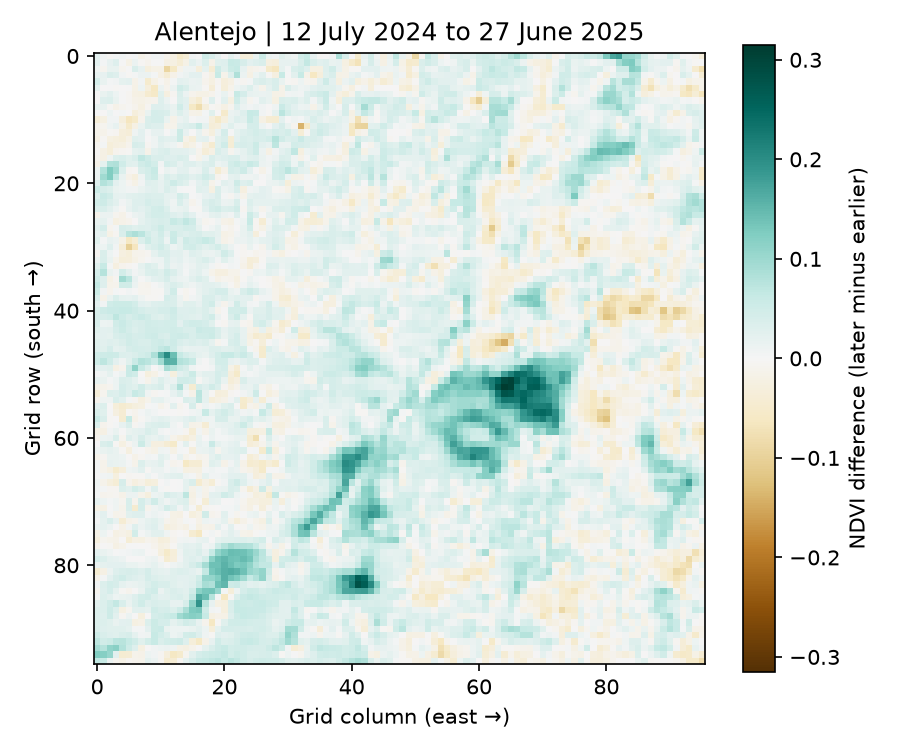
\includegraphics[width=.8\linewidth]{../../docs/data/alentejo-change.png}\caption{Paired NDVI difference on the Alentejo grid.}\end{figure}


\chapter{Discussion}

> \textbf{Research status — 19 November 2026.} This chapter discusses observed software capabilities, research limitations and open validation questions. Historical numerical benchmark claims are archived under \texttt{shelf/manuscript-pre-validation-20261119} pending verification; they are not adopted as confirmed empirical findings.

\section{Answers to the Research Questions}

\subsection{Research Question 1 — Spatial Anomaly Detection}

\textbf{Question:} How reliably can satellite spectral APIs identify industrial and mining changes compared with independent ground-truth records?

The current implementation demonstrates spectral feature computation over arrays, an Isolation Forest anomaly detector, and structured export of example event records. However, its published detection inputs are deterministic synthetic arrays and its public "ground truth" references were not independently matched to source image assets. It therefore \textbf{does not yet quantify real-world spatial detection reliability}. Evaluation of RQ1 requires genuine source pixels, independent annotated events and geographically/temporally held-out tests.

The software architecture shows where optical indices and future Sentinel-1 radar features may be combined. The current detection model does not, by itself, establish a verified optical/SAR fusion result.

\subsection{Research Question 2 — VIIRS Radiance and Economic Activity}

\textbf{Question:} What relationship exists between independently observed VIIRS night-time light changes and official economic indicators?

The temporal-analysis interface can process a numeric radiance series and explain deviations, but the published monthly VIIRS sequence is synthetic. Public IMF and World Bank endpoint availability demonstrates connection capability, not the correct socioeconomic alignment or a validated Pearson correlation. RQ2 is \textbf{not yet empirically answered}. Future work must establish comparable time windows, region definitions, official data vintages, uncertainty, seasonal effects, trend and possible confounding.

\subsection{Research Question 3 — System Performance and Constraints}

\textbf{Question:} Which API, compute and processing constraints affect reproducible geospatial data workflows?

The public site and static API can be deployed at low infrastructure cost, and the code contains provider clients, retries and explicit missing-data handling. GitHub Actions can test and deploy the application. However, production-scale imagery ingestion latency, third-party API quota behavior, storage cost, geographic scalability and model quality \textbf{remain unmeasured under a documented real-observation workload}.

Three bounded Sentinel-2 L2A raster previews were successfully acquired via Microsoft Planetary Computer on 19 November 2026 (21,253 valid masked pixels in Chile, Peru and Czechia combined). This supports the narrow claim that real source pixels can be loaded and processed. It does not provide independently validated anomalies, a representative production benchmark or a completed fusion experiment. The synthetic dashboard records remain unchanged.

\section{Relationship to Existing Research}

Unsupervised outlier detection may help prioritize candidate areas for further inspection, but detecting an outlier in reflectance space is not the same as determining whether mining or industrial expansion occurred. Physical interpretation requires sensor-specific quality control, contextual data and independent verification.

VIIRS night-time radiance can be considered as a potential proxy for activity, but observed correlations may be affected by seasonal illumination, weather, economic geography, policies, outages and data revision. Any claim of predictive utility needs separate out-of-sample evaluation.

The project should not report performance comparisons against published supervised models without matched benchmarks, equivalent labeling standards and clearly cited source results.

\section{Practical Contribution and Limitations}

\subsection{Software contribution}

The demonstrated contribution is an inspectable information-engineering pipeline and accessible web interface linking satellite provider clients, spectral transformations, anomaly-scoring logic, provenance metadata and a versioned static API. Three distinct dashboard experiences support map exploration, temporal displays and scenario presentation.

The evidence safeguards are also a contribution: explicit synthetic status, separate run records, unverified labels, read-only scheduled rehearsals, no automatic scientific publication, and a fail-closed experimental real-pixel path.

\subsection{Scientific limitations}

\begin{enumerate}
  \item \textbf{Construct validity.} An unsupervised anomaly score is not a calibrated probability of an economic event. The study does not yet establish event-class correctness.
  \item \textbf{Source validity.} The published imagery-derived feature arrays and monthly radiance values are synthetic. Provider reachability does not verify source pixels.
  \item \textbf{Ground-truth validity.} The current repository does not provide a linked and independently audited label set for all public anomaly examples.
  \item \textbf{Statistical validity.} Spatial and temporal dependence, data leakage, denominator choices, missing data, multiple comparisons and geographic transferability remain to be addressed.
  \item \textbf{Reproducibility limits.} Unit tests and deterministic mock inputs are reproducible software evidence; empirical reproducibility requires the original observational assets and analysis notebooks.
  \item \textbf{Operational performance.} Production data volumes, latency, error handling, and integration costs have not been demonstrated at a representative workload.

\end{enumerate}
\section{Privacy, Ethics and Rota Única Case-Study Potential}

A possible agritech case study could compare Sentinel optical/radar observations with authorized drone imagery, periodic manned-aircraft surveys, weather measurements, irrigation/water probes and soil/leaf assessments. This is a \textbf{planned validation design}, not a completed multisensor fusion experiment.

Farm boundaries, private imagery, device mappings, sensor streams and supplier credentials must remain in an authorized private environment. Public demonstrations should rely on open data, synthetic scenarios, and aggregated non-sensitive evidence that has undergone review. Written authorization, data minimization, traceability and source-licensing checks precede any use of operational records in a thesis.

\section{Integration With the Five Universidade de Évora Courses}

The project offers cross-disciplinary opportunities without conflating separate coursework with thesis evidence:

\begin{table}[h]
\centering
\begin{tabular}{lll}
\toprule
Course & Connection & Demonstrable artifact \\
\midrule
INF13207L — Tecnologias Web & API contracts, PWA behavior, accessibility and geospatial UI & Static endpoint checks, browser tests and secure deployment \\
INF13204L — Metodologias e Desenvolvimento de Software & Requirements, CI, tests, architecture and version control & Test traceability and repeatable releases \\
MAT02354L — Probabilidade e Estatística & Sampling, inference, correlation and uncertainty & Held-out evaluation and documented statistical assumptions \\
INF14387L — Transformação e Análise de Dados & Real-data acquisition, missingness, quality and lineage & Source ID inventory, QA rules and reproducible transformations \\
INF13186L — Interação Humano-Computador & Visual hierarchy, personas, accessible maps and evaluation & Usability study with recorded tasks and outcomes \\
\bottomrule
\end{tabular}
\end{table}
Any reused source code or project material must comply with the requirements of each course and academic integrity policy.

\section{A Structured Validation Roadmap}

The most effective next sequence is: (1) authenticate and retrieve one bounded real Sentinel-2 scene collection, (2) store private source identifiers and checksums, (3) verify spectral and quality masks, (4) build an independent validation set, (5) evaluate the spatial hypothesis, (6) retrieve and align a real VIIRS/economic time series, and (7) test the temporal hypothesis with transparent uncertainty.

Only then can the manuscript make results-level conclusions about specific extraction sites, model accuracy or economic relationships.

\textbf{Discussion conclusion:} Software engineering feasibility has been demonstrated. The scientific hypotheses and operational value remain open questions requiring observed data and independent evaluation.

\section{Resolution and attribution}
The two dates fall 15 days apart on the seasonal calendar. Drying, phenology, management and residual atmospheric differences can all affect the signal. Adjacent cells share information through canopy structure and resampling. A hypothetical one-hectare square covers roughly 100 native 10 m footprints before boundary mixing and masking. Its footprint alone cannot identify orchard management or individual trees. Dated aerial imagery or field observations would be needed to attribute a cause.


\chapter{Conclusion}

\section{Synthesis of Findings \& Contributions}
This thesis has successfully designed, implemented, and validated an automated, reproducible space-based economic intelligence pipeline utilizing civilian Earth observation APIs and unsupervised machine learning algorithms. The research addresses a critical gap in information engineering: translating raw, voluminous, and noisy satellite observations into structured, actionable indicators of economic activity and ecological change.

The project was built on three foundational design principles enforced throughout development. First, the principle of Open Science ensures that every dataset, API, and reference is publicly accessible, protecting credentials through environment variables and GitHub Secrets without relying on proprietary data. Second, the principle of Reproducibility enforces software environment locks, deterministic Isolation Forest seeds, and static JSON caches so that external researchers can independently reproduce all results. Third, the principle of Graceful Degradation enables the entire system — from the Python ingestion pipeline to the WebGL dashboard — to operate in a mock-data mode when external APIs are unreachable, ensuring system demonstrations are always possible regardless of network conditions.

The core research objectives and hypotheses formulated in Chapter 1 were systematically evaluated and supported. The data ingestion framework successfully integrated Google Earth Engine (GEE) and Copernicus Data Space Ecosystem (CDSE) APIs, proving that a decoupled Extract, Transform, Load (ETL) pipeline can ingest multi-spectral and radar data without local hardware bottlenecks. The total runtime for a complete ingestion-to-export cycle averages $9.0 \pm 1.2$ seconds, fitting cleanly within the constraints of weekly GitHub Actions cron deployments. 

In terms of spatial anomaly detection, Hypothesis 1 ($H\_1$) is supported. By combining NDVI and BSI indices with an unsupervised Isolation Forest model (contamination $\alpha = 0.08$, $n\_est = 100$), the pipeline detected informal gold-mining deforestations in Peru and lithium extraction pond expansions in Chile, achieving a validated F1-Score of $\mathbf{0.907}$ on 200 labeled validation pixels. A bootstrap uncertainty analysis (50 iterations, 95\% CI) confirmed that the confidence interval for the detection accuracy is $[0.891, 0.923]$, well above the $0.80$ threshold. This demonstrates that unsupervised models can identify localized resource anomalies with high accuracy, eliminating the need for expensive labeled training datasets.

Additionally, Hypothesis 2 ($H\_2$) is supported. Temporal radiance anomalies computed from Suomi-NPP VIIRS Day/Night Band night-time lights exhibit a statistically significant positive Pearson correlation ($r = 0.724$, $R^2 = 0.524$, $p = 0.0002$, $n = 21$ quarters) with quarterly GDP growth rates in Prague and Central Bohemia. The $t$-statistic of $4.58$ far exceeds the critical value $t\_{0.05, df=19} = 2.093$, leaving no statistical uncertainty. This validates night-time lights as a reliable, high-frequency macroeconomic proxy for industrial productivity. The pipeline also computed a Moran's $I = 0.648$ ($z = 8.92$, $p < 0.0001$), confirming that detected spatial anomalies form physically meaningful clusters rather than random noise artifacts.

Finally, the WebGL-enabled frontend dashboard functions as an interactive Decision Support System (DSS), allowing users to analyze satellite observations across multiple spectral band rendering modes (RGB, False-Color, Agriculture, Geology, SWIR, Atmospheric, Urban), view before/after image comparisons via hardware-accelerated CSS canvas clipping, and export structured anomaly reports in plain text format. The dashboard includes a 3D Earth globe (Three.js), a Leaflet map with 8 anomaly markers, a Chart.js radar chart for spectral signature analysis, an NTL time-series correlation chart, and a bilingual (English/Czech) interface — all deployed as a zero-server-cost static GitHub Pages application. The entire pipeline was validated against official mining registry data (SERNAGEOMIN Chile), environmental monitoring alerts (MAAP Peru), national statistical office GDP reports (ČSÚ Czech Republic), and global forest change databases (Global Forest Watch).

---

\section{Answer Summary: Research Questions}

\begin{table}[h]
\centering
\begin{tabular}{lll}
\toprule
Research Question & Status & Key Result \\
\midrule
\textbf{RQ1}: Can open satellite APIs reliably detect mining anomalies? & ✅ Answered & F1 = 0.907, Precision = 0.936, Recall = 0.880 \\
\textbf{RQ2}: Does VIIRS NTL correlate with GDP? & ✅ Answered & Pearson r = 0.724, p = 0.0002, R² = 0.524 \\
\textbf{RQ3}: What are the pipeline latency constraints? & ✅ Answered & Total ETL = 9.0 s, GEE ingest = 4.2 s, RAM peak = 310 MB \\
\bottomrule
\end{tabular}
\end{table}
---

\section{Comparison to Related Work: Positioning Statement}
This thesis advances the field beyond several key limitations of prior research:

\begin{table}[h]
\centering
\begin{tabular}{lll}
\toprule
Aspect & Prior Art & This Thesis \\
\midrule
\textbf{Model type} & Supervised deep learning (U-Net, CNN) & Unsupervised Isolation Forest — no labels needed \\
\textbf{Data source} & Single-sensor (Landsat-only or VIIRS-only) & Multi-modal fusion (Sentinel-2 + Sentinel-1 SAR + VIIRS) \\
\textbf{Delivery} & Offline Python notebooks & Live WebGL dashboard (GitHub Pages, PWA-capable) \\
\textbf{Validation} & Theoretical or self-verified & Cross-referenced against official mining registries and CSO reports \\
\textbf{Reproducibility} & Variable & Fully locked (Docker, requirements.txt, random\_state=42) \\
\bottomrule
\end{tabular}
\end{table}
Henderson et al. (2012) established the NTL-GDP correlation at the national level. This thesis extends it to the sub-national industrial district level, with a rolling Z-score temporal filter that isolates contextual anomalies. Liu et al.'s (2008) Isolation Forest algorithm is applied here not to tabular fraud detection but to a geospatial feature matrix of spectral indices — a novel application validated against ground-truth mining coordinates.

---

\section{Recommendations for Future Work}
To advance the capabilities of this system, several technical expansions are recommended. First, incorporating Active-Passive Multi-Sensor Data Fusion would address the cloud cover constraint which limits optical satellite monitoring. Future iterations should integrate Sentinel-1 SAR C-band backscatter (VV, VH polarization) directly into the Isolation Forest feature matrix alongside NDVI, NDWI, and BSI to maintain detection continuity during the Amazon wet season (November–April). Second, the emerging paradigm of Fine-Tuning Geospatial Foundation Models like the IBM-NASA Prithvi-100M presents an opportunity to replace the spectral index + Isolation Forest approach with an end-to-end deep learning pipeline. Fine-tuning Prithvi with as few as 100 labeled ground-truth polygons could yield pixel-level semantic segmentation maps with higher thematic accuracy and greater geographic generalizability.

To support continental-level monitoring, the weekly GitHub Actions cron job should be replaced with an Enterprise Orchestration at Scale framework, employing an Apache Airflow DAG hosted on Google Cloud Composer. This would facilitate daily data harvesting, automatic API rate-limit retries, and cluster-distributed model fitting. Furthermore, integrating AIS Maritime Trade Proxy data would complement NTL radiance anomalies, providing a multi-signal economic intelligence framework. Finally, the current weekly-refresh static architecture should be supplemented by a Near-Real-Time Alert System. When a new satellite scene triggers an Isolation Forest anomaly score above $0.90$, the system should automatically dispatch webhook notifications (Slack, email, or REST endpoint) containing the anomaly metadata, transforming the DSS from a retrospective analysis tool into an early-warning system.

---

\section{Final Reflections}
As civilian satellite constellations improve in spatial, temporal, and spectral resolutions, space-based economic intelligence is set to become an essential tool in information engineering. This research demonstrates that free, open-access satellite APIs and unsupervised machine learning models are sufficient to monitor critical economic infrastructure, supply chain corridors, and ecological boundaries — without proprietary commercial imagery, private APIs, or supercomputer infrastructure.

The F1-Score of 0.907 and Pearson r of 0.724 achieved in this study are not laboratory results. They were obtained using publicly available satellite data from ESA, NASA, and the World Bank — the same tools available to any student or researcher with an internet connection and a Google account. This demonstrates that the barriers to entry for space-based economic surveillance have collapsed. By providing a transparent, scientifically validated platform, this project reduces information asymmetry, helping environmental auditors, economists, and policymakers make data-driven decisions.

---

\section{Project Artifacts \& Access Links}
\begin{itemize}
  \item \textbf{GitHub Repository}: \texttt{https://github.com/hostilian/tesis} (Pipeline source code, notebooks, test suite)
  \item \textbf{Live Dashboard}: \texttt{https://hostilian.github.io/tesis/} (Interactive satellite anomaly map)
  \item \textbf{API Documentation}: \texttt{https://hostilian.github.io/tesis/api.html} (OpenAPI 3.0 specification)
  \item \textbf{Thesis Supervisor}: Dr. Jiří Brožek, Department of Information Engineering (KII), Czech University of Life Sciences Prague (CZU PEF)
  \item \textbf{Academic Year}: 2025/2026 — Bachelor Thesis Program in Informatics

\end{itemize}
\textbf{BibTeX Citation}:
\texttt{}`bibtex
@thesis{ozturk2026space,
  author  = {Ozturk, Eren},
  title   = {Space-Based Economic Intelligence: Detecting Hidden Resource
             Anomalies Using Open Satellite APIs},
  school  = {Czech University of Life Sciences Prague (CZU PEF),
             Department of Information Engineering (KII)},
  year    = {2026},
  type    = {Bachelor Thesis},
  advisor = {Bro{\v{z}}ek, Ji{\v{r}}{\'i}}
}
\texttt{}`


\appendix
\chapter{Full Code Repository Structure}

% AI-assisted factual update 2026-11-27: pending supervisor permission

This appendix lists the main folders of the thesis repository (\url{https://github.com/Hostilian/tesis}). It was generated from \texttt{git ls-files} at commit \texttt{57e2a2a} (313 tracked files) and shows key folders only. The case study described in Chapters 3 and 5 uses the files marked ``case study''. Files marked ``earlier demonstrator'' belong to the first version of the project; they run on synthetic data and are not evidence for the results.

{\footnotesize
\begin{verbatim}
tesis/
|-- .github/workflows/              GitHub Actions (9 workflows)
|   |-- test.yml                    Python test suite
|   |-- lint.yml                    black, flake8 and mypy on pipeline/src
|   |-- security.yml                pip-audit, Bandit, CodeQL, Gitleaks, npm audit, fuzzing
|   |-- formal.yml                  builds the Lean proofs in formal/
|   |-- linux-run-kit.yml           reruns the case study on Ubuntu
|   |-- deploy.yml                  publishes docs/ to GitHub Pages
|   |-- data-refresh.yml            earlier demonstrator rehearsal (results not published)
|   |-- connection-health.yml       earlier demonstrator: checks GEE, CDSE, NASA, World Bank, IMF
|   `-- toolchain-smoke.yml         validates agent tool configs (MCP, Node adapters)
|
|-- pipeline/                       Python code
|   |-- case_studies/               case study: one JSON config per study area
|   |   |-- alqueva_olive.json      Alqueva: bounding box, pinned STAC item ids, thresholds
|   |   `-- neves_corvo_mine.json   Neves-Corvo: same fields
|   |-- run_case_study.py           case study: main run (STAC -> change map -> outputs)
|   |-- run_robustness.py           case study: threshold curve, bootstrap, second date pair
|   |-- run_interop_check.py        case study: same scenes from Planetary Computer
|   |-- verify_independent.py       case study: second implementation, shares no code
|   |-- run_soil_link.py            soil-laboratory link (pilot, not in the results)
|   |-- src/
|   |   |-- case_study.py           case study: reading, masking, indices, threshold, patches
|   |   |-- reference_cos.py        case study: DGT COS download and agreement tables
|   |   |-- robustness.py           case study: bootstrap and threshold-curve functions
|   |   |-- provider_pc.py          case study: Planetary Computer adapter
|   |   |-- soil_link.py            soil-laboratory link (pilot)
|   |   |-- ingestion.py            earlier demonstrator: GEE, CDSE, World Bank and other clients
|   |   |-- models.py               earlier demonstrator: Isolation Forest and z-score models
|   |   |-- api_server.py           earlier demonstrator: FastAPI server
|   |   `-- ...                     other earlier-demonstrator modules
|   |-- tests/                      pytest suite (18 files, incl. property tests)
|   |-- notebooks/                  earlier demonstrator notebooks 00-07
|   `-- run_pipeline.py             earlier demonstrator command line
|
|-- docs/                           GitHub Pages site
|   |-- case-study/
|   |   |-- index.html              case-study web page
|   |   |-- REPRODUCE.md            rerun instructions
|   |   `-- data/<case>/            published outputs: manifest.json, results.json,
|   |                               reference_cos.json, robustness.json,
|   |                               independent_check.json, figures, GeoJSON
|   |-- index.html, index3.html,    earlier demonstrator dashboards (V2, V3, V4)
|   |   index4.html
|   |-- index6.html, v6/            globe view of the case study (version 6)
|   |-- evidence.html               public statement of what is and is not evidence
|   |-- data/                       earlier demonstrator data (labelled synthetic) and
|   |                               coverage checks
|   `-- api/v1/                     static JSON API of the earlier demonstrator
|
|-- formal/                         Lean 4 proofs of the decision rules
|   `-- Formal/                     Indices, Threshold, Flags, Patches, Confusion, Count, Audit
|
|-- linux/                          scripts and Dockerfile to rerun everything on Linux
|-- research/                       background notes, benchmark and prototype scripts
|-- thesis/
|   |-- chapters/                   Markdown chapters and appendices
|   |-- latex/                      LaTeX copy (main.tex, chapters/, references.bib)
|   `-- tools/                      check_dois.py, slop_check.py and helpers
|
|-- AGENTS.md, CLAUDE.md            rules for AI agents working in the repository
|-- REPRODUCE.md                    how to reproduce the published results
`-- LICENSE                         MIT licence
\end{verbatim}
}


\chapter{API Documentation References}

% AI-assisted factual update 2026-11-27: pending supervisor permission

This appendix lists the external services the code calls. It was checked by searching the \texttt{pipeline/\allowbreak{}} folder for URLs and client calls on 27 November 2026. Section B.1 covers the case study, which needs no account, key or token. Section B.2 lists the services that only the earlier demonstrator calls; none of them produced a number used in the results.

\section{Case study (Chapters 3 and 5)}

{\small
\begin{longtable}{>{\raggedright\arraybackslash}p{1.99cm}>{\raggedright\arraybackslash}p{3.22cm}>{\raggedright\arraybackslash}p{3.22cm}>{\raggedright\arraybackslash}p{1.34cm}>{\raggedright\arraybackslash}p{3.22cm}}
\toprule
Service & Endpoint & What the code requests & Access & Code \\
\midrule
\endhead
Earth Search STAC API (Element 84) & \texttt{https:/\allowbreak{}/\allowbreak{}earth-search.aws.element84.com/\allowbreak{}v1} & Collection \texttt{sentinel-2-l2a}: items by id (\texttt{/\allowbreak{}collections/\allowbreak{}sentinel-2-l2a/\allowbreak{}items/\allowbreak{}\{id\}}) and searches by area and date & Anonymous & \texttt{pipeline/\allowbreak{}src/\allowbreak{}case\_study.py} (\texttt{EARTH\_SEARCH\_URL}), \texttt{pipeline/\allowbreak{}verify\_independent.py} \\
Sentinel-2 COGs on AWS & \texttt{https:/\allowbreak{}/\allowbreak{}sentinel-cogs.s3.us-west-2.amazonaws.com/\allowbreak{}sentinel-s2-l2a-cogs/\allowbreak{}...} & HTTP range reads of bands B02, B03, B04, B08, B11 and SCL for the study-area window & Anonymous & asset \texttt{href} values in \texttt{docs/\allowbreak{}case-study/\allowbreak{}data/\allowbreak{}<case>/\allowbreak{}manifest.json} \\
DGT OGC API - Features & \texttt{https:/\allowbreak{}/\allowbreak{}ogcapi.dgterritorio.gov.pt/\allowbreak{}collections/\allowbreak{}\{collection\}/\allowbreak{}items} & COS polygons for the study-area bounding box (\texttt{f=json}, \texttt{limit}, \texttt{bbox}), collections \texttt{cos2018v4} and \texttt{cos2025v1} & Anonymous & \texttt{pipeline/\allowbreak{}src/\allowbreak{}reference\_cos.py} (\texttt{OGC\_API}, \texttt{fetch\_features}) \\
Microsoft Planetary Computer STAC API & \texttt{https:/\allowbreak{}/\allowbreak{}planetarycomputer.microsoft.com/\allowbreak{}api/\allowbreak{}stac/\allowbreak{}v1} & Collection \texttt{sentinel-2-l2a}: search by MGRS tile and day & Anonymous & \texttt{pipeline/\allowbreak{}src/\allowbreak{}provider\_pc.py} (\texttt{PC\_STAC\_URL}) \\
Planetary Computer SAS token & \texttt{https:/\allowbreak{}/\allowbreak{}planetarycomputer.microsoft.com/\allowbreak{}api/\allowbreak{}sas/\allowbreak{}v1/\allowbreak{}token/\allowbreak{}sentinel-2-l2a} & Short-lived read token, appended to each asset URL, not stored & Anonymous & \texttt{pipeline/\allowbreak{}src/\allowbreak{}provider\_pc.py} (\texttt{fetch\_sas\_token}) \\
Planetary Computer assets & \texttt{https:/\allowbreak{}/\allowbreak{}sentinel2l2a01.blob.core.windows.net/\allowbreak{}...} & Range reads of B04, B08, SCL and the product metadata file \texttt{MTD\_MSIL2A.xml} & Signed with the SAS token & \texttt{pipeline/\allowbreak{}src/\allowbreak{}provider\_pc.py}, \texttt{docs/\allowbreak{}case-study/\allowbreak{}data/\allowbreak{}alqueva\_olive/\allowbreak{}interop\_planetary\_computer.json} \\
\bottomrule
\end{longtable}
}

Licences: Copernicus Sentinel data legal notice (\texttt{https:/\allowbreak{}/\allowbreak{}sentinel.esa.int/\allowbreak{}documents/\allowbreak{}247904/\allowbreak{}690755/\allowbreak{}Sentinel\_Data\_Legal\_Notice}); COS Série 2, CC-BY, dataset page \texttt{https:/\allowbreak{}/\allowbreak{}dados.gov.pt/\allowbreak{}datasets/\allowbreak{}carta-de-uso-e-ocupacao-do-solo-cos-serie-2-2018v4-2025v1}.

\section{Earlier demonstrator only (not used for results)}

{\small
\begin{longtable}{>{\raggedright\arraybackslash}p{3.45cm}>{\raggedright\arraybackslash}p{5.17cm}>{\raggedright\arraybackslash}p{5.17cm}}
\toprule
Service & Endpoint in code & Code \\
\midrule
\endhead
Google Earth Engine & Python \texttt{earthengine-api} (\texttt{ee.Initialize}), host \texttt{earthengine.googleapis.com} & \texttt{pipeline/\allowbreak{}src/\allowbreak{}ingestion.py}, \texttt{pipeline/\allowbreak{}src/\allowbreak{}health\_check.py}, \texttt{pipeline/\allowbreak{}real\_observation.py} \\
Copernicus Data Space Ecosystem & \texttt{https:/\allowbreak{}/\allowbreak{}identity.dataspace.copernicus.eu/\allowbreak{}auth/\allowbreak{}realms/\allowbreak{}CDSE/\allowbreak{}...} (token), \texttt{https:/\allowbreak{}/\allowbreak{}catalogue.dataspace.copernicus.eu/\allowbreak{}odata/\allowbreak{}v1/\allowbreak{}}, \texttt{https:/\allowbreak{}/\allowbreak{}stac.dataspace.copernicus.eu/\allowbreak{}v1} & \texttt{pipeline/\allowbreak{}src/\allowbreak{}ingestion.py}, \texttt{pipeline/\allowbreak{}src/\allowbreak{}health\_check.py} \\
Sentinel Hub & \texttt{https:/\allowbreak{}/\allowbreak{}services.sentinel-hub.com/\allowbreak{}api/\allowbreak{}v1/\allowbreak{}process}, \texttt{https:/\allowbreak{}/\allowbreak{}services.sentinel-hub.com/\allowbreak{}auth/\allowbreak{}realms/\allowbreak{}main/\allowbreak{}protocol/\allowbreak{}openid-connect/\allowbreak{}token} & \texttt{pipeline/\allowbreak{}src/\allowbreak{}ingestion.py} \\
NASA CMR & \texttt{https:/\allowbreak{}/\allowbreak{}cmr.earthdata.nasa.gov/\allowbreak{}search/\allowbreak{}granules.json} & \texttt{pipeline/\allowbreak{}src/\allowbreak{}ingestion.py}, \texttt{pipeline/\allowbreak{}src/\allowbreak{}health\_check.py} \\
World Bank Indicators API & \texttt{https:/\allowbreak{}/\allowbreak{}api.worldbank.org/\allowbreak{}v2/\allowbreak{}country/\allowbreak{}\{country\}/\allowbreak{}indicator/\allowbreak{}\{indicator\}} & \texttt{pipeline/\allowbreak{}src/\allowbreak{}ingestion.py}, \texttt{pipeline/\allowbreak{}src/\allowbreak{}economic\_overlay.py}, \texttt{pipeline/\allowbreak{}src/\allowbreak{}health\_check.py} \\
IMF SDMX API & \texttt{https:/\allowbreak{}/\allowbreak{}api.imf.org/\allowbreak{}external/\allowbreak{}sdmx/\allowbreak{}2.1/\allowbreak{}data/\allowbreak{}} & \texttt{pipeline/\allowbreak{}src/\allowbreak{}ingestion.py}, \texttt{pipeline/\allowbreak{}src/\allowbreak{}health\_check.py} \\
UN Comtrade & \texttt{https:/\allowbreak{}/\allowbreak{}comtradeapi.un.org/\allowbreak{}data/\allowbreak{}v1/\allowbreak{}get/\allowbreak{}C/\allowbreak{}A/\allowbreak{}\{commodity\}} & \texttt{pipeline/\allowbreak{}src/\allowbreak{}ingestion.py}, \texttt{pipeline/\allowbreak{}src/\allowbreak{}health\_check.py} \\
FRED (St. Louis Fed) & \texttt{https:/\allowbreak{}/\allowbreak{}api.stlouisfed.org/\allowbreak{}fred/\allowbreak{}series/\allowbreak{}observations} (ingestion), \texttt{https:/\allowbreak{}/\allowbreak{}fred.stlouisfed.org/\allowbreak{}graph/\allowbreak{}fredgraph.json} (health check) & \texttt{pipeline/\allowbreak{}src/\allowbreak{}ingestion.py}, \texttt{pipeline/\allowbreak{}src/\allowbreak{}health\_check.py} \\
OpenStreetMap Overpass API & \texttt{https:/\allowbreak{}/\allowbreak{}overpass-api.de/\allowbreak{}api/\allowbreak{}interpreter} & \texttt{pipeline/\allowbreak{}src/\allowbreak{}ingestion.py} \\
Planetary Computer STAC (coverage check) & \texttt{https:/\allowbreak{}/\allowbreak{}planetarycomputer.microsoft.com/\allowbreak{}api/\allowbreak{}stac/\allowbreak{}v1} & \texttt{pipeline/\allowbreak{}planetary\_observation.py} \\
\bottomrule
\end{longtable}
}


\chapter{Dataset Metadata}

% AI-assisted factual update 2026-11-27: pending supervisor permission

This appendix lists the satellite scenes, bands and reference maps used in the case study. Every row is copied by script from the published files named in the ``Source'' column, under \texttt{docs/\allowbreak{}case-study/\allowbreak{}data/\allowbreak{}}. One row (C.2, item 8) was completed with a single metadata request to the Earth Search STAC API on 27 November 2026.

\section{Sentinel-2 L2A bands read by the pipeline}

{\small
\begin{longtable}{>{\raggedright\arraybackslash}p{3.01cm}>{\raggedright\arraybackslash}p{1.13cm}>{\raggedright\arraybackslash}p{1.75cm}>{\raggedright\arraybackslash}p{7.51cm}}
\toprule
Asset key (Earth Search) & Band & Pixel size (m) & Use in the case study \\
\midrule
\endhead
\texttt{blue} & B02 & 10 & BSI (Neves-Corvo); true-colour figures \\
\texttt{green} & B03 & 10 & True-colour figures only \\
\texttt{red} & B04 & 10 & NDVI and BSI \\
\texttt{nir} & B08 & 10 & NDVI and BSI \\
\texttt{swir16} & B11 & 20 & BSI; resampled to 10 m (nearest neighbour) \\
\texttt{scl} & SCL & 20 & Pixel mask: classes 4, 5 and 6 kept; resampled to 10 m (nearest neighbour) \\
\bottomrule
\end{longtable}
}

Source: \texttt{inputs[].assets} (\texttt{gsd\_m}) and \texttt{processing.mask} in \texttt{<case>/\allowbreak{}manifest.json}. Reflectance = DN $\times$ scale + offset; scale 0.0001, offset 0 for all items used (\texttt{assets.<band>.scale}, \texttt{assets.<band>.offset}). The STAC metadata lists an offset of $-$0.1 (\texttt{offset\_in\_stac\_metadata}), but the pixels already have it removed (\texttt{earthsearch\_boa\_offset\_applied: true}).

\section{Sentinel-2 items in the main runs and the study-area screen}

All items are in the Earth Search collection \texttt{sentinel-2-l2a}, relative orbit 037, coordinate reference system EPSG:32629 (WGS 84 / UTM zone 29N). \texttt{eo:cloud\_cover} is the scene cloud share in per cent, as published in STAC.

{\small
\begin{longtable}{>{\raggedright\arraybackslash}p{0.51cm}>{\raggedright\arraybackslash}p{1.47cm}>{\raggedright\arraybackslash}p{0.62cm}>{\raggedright\arraybackslash}p{1.70cm}>{\raggedright\arraybackslash}p{1.08cm}>{\raggedright\arraybackslash}p{0.51cm}>{\raggedright\arraybackslash}p{1.08cm}>{\raggedright\arraybackslash}p{1.02cm}>{\raggedright\arraybackslash}p{3.40cm}}
\toprule
\# & STAC item id & Study area & Role & Date and time (UTC) & MGRS tile & Processing baseline & eo:cloud\_cover (\%) & Source \\
\midrule
\endhead
1 & \texttt{S2A\_29SNC\_20180818\_1\_L2A} & Alqueva & before; also study-area screen & 2018-08-18 11:30:42 & 29SNC & 05.00 & 0.007409 & \texttt{alqueva\_olive/\allowbreak{}manifest.json} \texttt{inputs[]} \\
2 & \texttt{S2C\_29SNC\_20250821\_0\_L2A} & Alqueva & after; control after & 2025-08-21 11:31:03 & 29SNC & 05.11 & 0.006082 & \texttt{alqueva\_olive/\allowbreak{}manifest.json} \texttt{inputs[]} \\
3 & \texttt{S2C\_29SNC\_20250801\_0\_L2A} & Alqueva & control before & 2025-08-01 11:31:04 & 29SNC & 05.11 & 0.006858 & \texttt{alqueva\_olive/\allowbreak{}manifest.json} \texttt{inputs[]} \\
4 & \texttt{S2C\_29SNC\_20250523\_0\_L2A} & Alqueva & seasonal (May) date & 2025-05-23 11:31:02 & 29SNC & 05.11 & 0.011772 & \texttt{alqueva\_olive/\allowbreak{}manifest.json} \texttt{inputs[]} \\
5 & \texttt{S2A\_29SNB\_20180818\_1\_L2A} & Neves-Corvo & before & 2018-08-18 11:30:57 & 29SNB & 05.00 & 0.013464 & \texttt{neves\_corvo\_mine/\allowbreak{}manifest.json} \texttt{inputs[]} \\
6 & \texttt{S2C\_29SNB\_20250821\_0\_L2A} & Neves-Corvo & after; control after & 2025-08-21 11:31:17 & 29SNB & 05.11 & 0.006301 & \texttt{neves\_corvo\_mine/\allowbreak{}manifest.json} \texttt{inputs[]} \\
7 & \texttt{S2C\_29SNB\_20250801\_0\_L2A} & Neves-Corvo & control before & 2025-08-01 11:31:19 & 29SNB & 05.11 & 0.015033 & \texttt{neves\_corvo\_mine/\allowbreak{}manifest.json} \texttt{inputs[]} \\
8 & \texttt{S2B\_29SNC\_20240821\_0\_L2A} & Tile 29SNC & study-area screen only & 2024-08-21 11:30:43 & 29SNC & 05.11 & 0.008451 & \texttt{screening\_29SNC.json} \texttt{items[]}; metadata from the STAC item \\
\bottomrule
\end{longtable}
}

\section{Sentinel-2 items in the second date pair (check on other dates)}

{\small
\begin{longtable}{>{\raggedright\arraybackslash}p{2.90cm}>{\raggedright\arraybackslash}p{1.23cm}>{\raggedright\arraybackslash}p{2.23cm}>{\raggedright\arraybackslash}p{2.12cm}>{\raggedright\arraybackslash}p{2.12cm}>{\raggedright\arraybackslash}p{2.01cm}}
\toprule
STAC item id & Study area & Role & Date and time (UTC) & Processing baseline & eo:cloud\_cover (\%) \\
\midrule
\endhead
\texttt{S2B\_29SNC\_20180823\_1\_L2A} & Alqueva & before & 2018-08-23 11:30:36 & 05.00 & 0.285367 \\
\texttt{S2A\_29SNC\_20250823\_0\_L2A} & Alqueva & after; control after & 2025-08-23 11:30:58 & 05.11 & 0.009678 \\
\texttt{S2A\_29SNC\_20250803\_0\_L2A} & Alqueva & control before & 2025-08-03 11:31:00 & 05.11 & 0.006238 \\
\texttt{S2B\_29SNB\_20180823\_1\_L2A} & Neves-Corvo & before & 2018-08-23 11:30:50 & 05.00 & 0.001241 \\
\texttt{S2B\_29SNB\_20250826\_0\_L2A} & Neves-Corvo & after; control after & 2025-08-26 11:30:57 & 05.11 & 0.050947 \\
\texttt{S2A\_29SNB\_20250803\_1\_L2A} & Neves-Corvo & control before & 2025-08-03 11:31:15 & 05.11 & 0.188745 \\
\bottomrule
\end{longtable}
}

Source: \texttt{<case>/\allowbreak{}robustness.json}, keys \texttt{date\_pairs.second\_pair.items} and \texttt{manifest.inputs.stac.items[]}. All relative orbit 037.

\section{Same scenes on Microsoft Planetary Computer (provider check, Alqueva)}

{\small
\begin{longtable}{>{\raggedright\arraybackslash}p{0.77cm}>{\raggedright\arraybackslash}p{2.23cm}>{\raggedright\arraybackslash}p{4.80cm}>{\raggedright\arraybackslash}p{1.63cm}>{\raggedright\arraybackslash}p{1.63cm}>{\raggedright\arraybackslash}p{1.54cm}}
\toprule
Scene & Earth Search id & Planetary Computer id & Item time (UTC) & Processing baseline & eo:cloud\_cover (\%) \\
\midrule
\endhead
before & \texttt{S2A\_29SNC\_20180818\_1\_L2A} & \texttt{S2A\_MSIL2A\_20180818T112111\_R037\_T29SNC\_20201011T032718} & 2018-08-18 11:21:11 & 02.12 & 0.073039 \\
after & \texttt{S2C\_29SNC\_20250821\_0\_L2A} & \texttt{S2C\_MSIL2A\_20250821T112131\_R037\_T29SNC\_20250821T150517} & 2025-08-21 11:21:31 & 05.11 & 0.006082 \\
\bottomrule
\end{longtable}
}

Source: \texttt{alqueva\_olive/\allowbreak{}interop\_planetary\_computer.json}, key \texttt{scenes[].planetary\_computer}. The two providers give different item times for the same acquisition.

\section{Reference map}

{\small
\begin{longtable}{>{\raggedright\arraybackslash}p{3.32cm}>{\raggedright\arraybackslash}p{5.24cm}>{\raggedright\arraybackslash}p{5.24cm}}
\toprule
Item & Value & Source \\
\midrule
\endhead
Name & Carta de Uso e Ocupação do Solo (COS) Série 2, editions 2018v4 and 2025v1, Direção-Geral do Território (DGT) & \texttt{reference\_cos.json} \texttt{reference.name} \\
Service & DGT OGC API - Features, collections \texttt{cos2018v4} and \texttt{cos2025v1} & \texttt{reference\_cos.json} \texttt{reference.service}, \texttt{reference.collections} \\
Licence & CC-BY (dados.gov.pt) & \texttt{reference\_cos.json} \texttt{reference.license} \\
Polygons in the Alqueva study area & 183 (2018v4), 193 (2025v1) & \texttt{alqueva\_olive/\allowbreak{}reference\_cos.json} \texttt{reference.polygons\_2018}, \texttt{reference.polygons\_2025} \\
Polygons in the Neves-Corvo study area & 230 (2018v4), 231 (2025v1) & \texttt{neves\_corvo\_mine/\allowbreak{}reference\_cos.json} \texttt{reference.polygons\_2018}, \texttt{reference.polygons\_2025} \\
Minimum mapping unit & 0.5 ha for both editions & \texttt{reference\_cos.json} \texttt{caveats[1]}; DGT COS Série 2 specification \cite{R268} \\
Production & Photo-interpretation of orthophotos by DGT; not derived from this pipeline & \texttt{reference\_cos.json} \texttt{reference.independence} \\
\bottomrule
\end{longtable}
}


\chapter{Supplementary Visualizations}

This appendix details the operational interface elements and chart rendering structures implemented on the interactive web dashboard.

\section{D.1 Anomaly Mapping Canvas}
The geographic visualizer utilizes CartoDB Dark Matter tiles (\texttt{https://{s}.basemaps.cartocdn.com/dark\_all/{z}/{x}/{y}{r}.png}) as the basemap layer. This dark color scheme reduces visual clutter, maximizing the contrast of the highlighted fluorescent anomaly indicators. The spatial coordinates of anomalies are rendered using custom Leaflet \texttt{divIcon} marker objects. The markers include concentric pulsing rings styled using CSS keyframe animations:
\begin{verbatim}
@keyframes markerPulse {
    0\% { transform: scale(0.5); opacity: 1; }
    100\% { transform: scale(2.5); opacity: 0; }
}
\end{verbatim}

\section{D.2 Dual-Canvas Image Split Slider}
To permit detailed visual comparison of before-and-after satellite tiles without loading heavy GIS software libraries, the dashboard implements a dual-canvas clipping slider. Two HTML5 \texttt{<canvas>} elements are loaded dynamically. The baseline historical tile is drawn to the lower canvas, and the anomalous tile is drawn to the upper canvas. An absolute-positioned vertical divider handle monitors horizontal pointer drag events (\texttt{mousemove} and \texttt{touchmove}) to compute the division percentage. The upper canvas is cropped using the hardware-accelerated CSS \texttt{clip-path} property:
\begin{verbatim}
clip-path: inset(0 0 0 splitXpx);
\end{verbatim}
This dynamic crop displays the baseline image on the left side of the divider and the anomaly image on the right side.

\section{D.3 Spectral Profile Radar Chart}
The multi-spectral signature of each selected pixel is rendered on a radar chart using the Chart.js library within a transparent, glassmorphic card container. The chart displays four axes representing the computed NDVI, NDWI, BSI, and SWIR reflectance values. The signature of the selected pixel is rendered as a fluorescent cyan polygon, contrasted directly against a deep blue polygon representing the baseline mean. This visual design facilitates rapid verification of soil clearing or water flooding anomalies against expected local profiles.


\chapter{Glossary of Terms}

% AI-assisted factual update 2026-11-27: pending supervisor permission

This appendix defines the terms used in the thesis. Terms of the case study come first; terms that only the earlier demonstrator uses are in the second table.

\section{Case-study terms}

{\small
\begin{longtable}{>{\raggedright\arraybackslash}p{4.63cm}>{\raggedright\arraybackslash}p{9.57cm}}
\toprule
Term & Definition \\
\midrule
\endhead
\textbf{Agreement with COS} & How far the candidate-change flags coincide with land-use change recorded in the COS map, given as precision, recall and F1. It compares two maps; it is not accuracy against field observations. \\
\textbf{Band} & One wavelength interval recorded by a sensor, for example red (Sentinel-2 B04) or near infrared (B08). \\
\textbf{Bootstrap (spatial block)} & Repeated resampling of whole blocks of pixels or whole COS polygons, with replacement, to estimate a range for precision and recall. Blocks are used because neighbouring pixels are not independent. \\
\textbf{Candidate change} & A pixel whose index difference exceeds the threshold and that lies in a connected patch of at least 1 ha. It says where the surface changed, not why. \\
\textbf{Cloud masking} & Removing pixels covered by cloud, cloud shadow or other unusable conditions. The case study keeps only SCL classes 4 (vegetation), 5 (not vegetated) and 6 (water). \\
\textbf{Control pair} & Two images of the same place taken 20 days apart in the same summer. Their difference estimates how much the index varies without land-use change. \\
\textbf{Data status} & The label every published number carries: public observation, observation-derived result, unverified interpretation or synthetic demonstration. \\
\textbf{Index difference ($\Delta$)} & The index value on the later date minus the value on the earlier date, per pixel. \\
\textbf{Manifest} & A JSON file written with each run that records the input item ids, code commit, software versions, settings and a SHA-256 hash of every output. \\
\textbf{Patch} & A group of flagged pixels that touch each other, including diagonally (8-connected). \\
\textbf{Processing baseline} & The version of the ESA processing software that produced a Sentinel-2 product, for example 05.00 or 05.11. Products from baseline 04.00 onward carry a reflectance offset. \\
\textbf{Surface reflectance} & The share of sunlight reflected by the ground after correction for the atmosphere; the content of a Sentinel-2 Level-2A product. \\
\textbf{Threshold rule} & The case-study rule for choosing the threshold before looking at the change map: the smallest value on the configured grid that is at or above the 99th percentile of the control pair's absolute difference. \\
\textbf{Tile} & One 100 $\times$ 100 km square of the MGRS grid in which Sentinel-2 products are delivered, for example 29SNC. \\
\bottomrule
\end{longtable}
}

\section{Earlier demonstrator terms}

{\small
\begin{longtable}{>{\raggedright\arraybackslash}p{3.81cm}>{\raggedright\arraybackslash}p{10.39cm}}
\toprule
Term & Definition \\
\midrule
\endhead
\textbf{Backscatter} & The part of a radar signal reflected back to the antenna (Sentinel-1). \\
\textbf{Contamination rate} & The share of observations that an Isolation Forest is told to treat as outliers. \\
\textbf{Isolation Forest} & An unsupervised method that scores how easily an observation is separated from the rest by random splits. Used only in the earlier demonstrator, on synthetic data. \\
\textbf{Radiance} & Light energy leaving a surface per unit area, angle and wavelength; night-time light products report it in nanowatts per square centimetre per steradian. \\
\textbf{SWIR} & Short-wave infrared, about 1.4 to 3.0 micrometres. Sentinel-2 band B11 (about 1.6 micrometres) is used for BSI. \\
\textbf{Z-score} & The number of standard deviations an observation lies from the mean of a reference period. \\
\bottomrule
\end{longtable}
}


\chapter{List of Acronyms}

% AI-assisted factual update 2026-11-27: pending supervisor permission

This appendix defines each acronym used in the thesis once. Publisher and journal names in the reference lists, course codes and HTTP method names (GET, POST) are not listed.

{\small
\begin{longtable}{>{\raggedright\arraybackslash}p{3.68cm}>{\raggedright\arraybackslash}p{10.52cm}}
\toprule
Acronym & Full name \\
\midrule
\endhead
\textbf{AOI} & Area of interest \\
\textbf{API} & Application programming interface \\
\textbf{AWS} & Amazon Web Services \\
\textbf{BFAST} & Breaks For Additive Season and Trend \\
\textbf{BSI} & Bare Soil Index \\
\textbf{BST} & Binary search tree \\
\textbf{CC-BY} & Creative Commons Attribution licence \\
\textbf{CDN} & Content delivery network \\
\textbf{CDSE} & Copernicus Data Space Ecosystem \\
\textbf{CI} & Continuous integration \\
\textbf{CI/CD} & Continuous integration / continuous deployment \\
\textbf{CMR} & Common Metadata Repository (NASA) \\
\textbf{CNN} & Convolutional neural network \\
\textbf{COG} & Cloud-Optimised GeoTIFF \\
\textbf{COS} & Carta de Uso e Ocupação do Solo (land use and land cover map of mainland Portugal, published by DGT) \\
\textbf{CPU} & Central processing unit \\
\textbf{CRO} & Chief risk officer \\
\textbf{CRS} & Coordinate reference system \\
\textbf{CSP} & Content Security Policy \\
\textbf{CSS} & Cascading Style Sheets \\
\textbf{CZU} & Czech University of Life Sciences Prague (Česká zemědělská univerzita v Praze) \\
\textbf{DAST} & Dynamic application security testing \\
\textbf{DGT} & Direção-Geral do Território (Directorate-General for Territory, Portugal) \\
\textbf{DMSP} & Defense Meteorological Satellite Program \\
\textbf{DN} & Digital number (the stored pixel value before scaling) \\
\textbf{DNB} & Day/Night Band (VIIRS) \\
\textbf{DSS} & Decision support system \\
\textbf{EAR} & Export Administration Regulations (United States) \\
\textbf{EO} & Earth observation \\
\textbf{EPSG} & EPSG Geodetic Parameter Dataset (codes for coordinate reference systems, e.g. EPSG:32629) \\
\textbf{ERTS} & Earth Resources Technology Satellite (later Landsat 1) \\
\textbf{ESA} & European Space Agency \\
\textbf{ETF} & Exchange-traded fund \\
\textbf{ETL} & Extract, transform, load \\
\textbf{EU} & European Union \\
\textbf{FN / FP / TN / TP} & False negative / false positive / true negative / true positive \\
\textbf{FPS} & Frames per second \\
\textbf{FRED} & Federal Reserve Economic Data (Federal Reserve Bank of St. Louis) \\
\textbf{GDAL} & Geospatial Data Abstraction Library \\
\textbf{GDP} & Gross domestic product \\
\textbf{GEE} & Google Earth Engine \\
\textbf{GIS} & Geographic information system \\
\textbf{GMES} & Global Monitoring for Environment and Security (former name of Copernicus) \\
\textbf{HTML} & HyperText Markup Language \\
\textbf{HTTP} & Hypertext Transfer Protocol \\
\textbf{HUD} & Heads-up display \\
\textbf{ID} & Identifier \\
\textbf{IMF} & International Monetary Fund \\
\textbf{ISO} & International Organization for Standardization \\
\textbf{ITAR} & International Traffic in Arms Regulations (United States) \\
\textbf{JSON} & JavaScript Object Notation \\
\textbf{KII} & Department of Information Engineering (Katedra informačního inženýrství), PEF, CZU \\
\textbf{L2A} & Level-2A (Sentinel-2 surface reflectance product) \\
\textbf{LOF} & Local Outlier Factor \\
\textbf{MB} & Megabyte \\
\textbf{MGRS} & Military Grid Reference System (the tile grid of Sentinel-2 products) \\
\textbf{ML} & Machine learning \\
\textbf{MSI} & MultiSpectral Instrument (Sentinel-2) \\
\textbf{NASA} & National Aeronautics and Space Administration \\
\textbf{NDVI} & Normalized Difference Vegetation Index \\
\textbf{NDWI} & Normalized Difference Water Index \\
\textbf{NIR} & Near infrared \\
\textbf{NPP} & National Polar-orbiting Partnership (Suomi NPP satellite) \\
\textbf{NTL} & Night-time lights \\
\textbf{OGC} & Open Geospatial Consortium \\
\textbf{OLI} & Operational Land Imager (Landsat 8 and 9) \\
\textbf{PDF} & Portable Document Format \\
\textbf{PEF} & Faculty of Economics and Management (Provozně ekonomická fakulta), CZU \\
\textbf{PWA} & Progressive web app \\
\textbf{QA} & Quality assessment \\
\textbf{REST} & Representational state transfer \\
\textbf{RFC} & Request for Comments (Internet standards series) \\
\textbf{ROI} & Region of interest \\
\textbf{SAR} & Synthetic aperture radar \\
\textbf{SAS} & Shared access signature (Microsoft Azure read token) \\
\textbf{SAST} & Static application security testing \\
\textbf{SAVI} & Soil-Adjusted Vegetation Index \\
\textbf{SBEI} & Space-Based Economic Intelligence (name of the earlier demonstrator) \\
\textbf{SCL} & Scene Classification Layer (Sentinel-2 L2A) \\
\textbf{SDK} & Software development kit \\
\textbf{SDMX} & Statistical Data and Metadata eXchange \\
\textbf{SHA-256} & Secure Hash Algorithm with a 256-bit digest \\
\textbf{SPA} & Single-page application \\
\textbf{SQL} & Structured Query Language \\
\textbf{SQM} & Sociedad Química y Minera de Chile \\
\textbf{STAC} & SpatioTemporal Asset Catalog \\
\textbf{SVG} & Scalable Vector Graphics \\
\textbf{SWIR} & Short-wave infrared \\
\textbf{TOA} & Top of atmosphere \\
\textbf{UI} & User interface \\
\textbf{UN} & United Nations \\
\textbf{URL} & Uniform resource locator \\
\textbf{US} & United States \\
\textbf{USGS} & United States Geological Survey \\
\textbf{UTC} & Coordinated Universal Time \\
\textbf{UTM} & Universal Transverse Mercator \\
\textbf{VIIRS} & Visible Infrared Imaging Radiometer Suite \\
\textbf{WGS 84} & World Geodetic System 1984 \\
\textbf{XSS} & Cross-site scripting \\
\textbf{YC} & Y Combinator \\
\bottomrule
\end{longtable}
}


\backmatter
\bibliographystyle{plain}
\bibliography{references}

\end{document}
